\documentclass{article}
\usepackage{geometry}
\usepackage{listings}
\usepackage{amsmath}
\usepackage{amsfonts}
\usepackage{graphicx}
\usepackage{caption}
\usepackage{subcaption}
\usepackage{float}
\usepackage{hyperref}

\title{Solving the Navier-Stokes Equations: A Finite Element Approach}
\author{ Matteo Cenzato, Giuseppe Pisante, Arianna Procaccio}
\date{\today}

\begin{document}
\maketitle

\begin{figure}[H]
    \centering
    \includegraphics[width=0.4\linewidth]{20151029123608!Logo_Politecnico_Milano.png}
    \label{fig:enter-label}
\end{figure}



\newpage
\tableofcontents


\section*{Introduction}

This report aims to solve the unsteady, incompressible Navier-Stokes equations using the finite element method. The focus is to simulate the benchmark problem "flow past a cylinder" in two and three dimensions considering different values of the Reynolds number (\(Re \leq 200\)).



The report will discuss the obtained results, the methods employed, their stability and accuracy, and the algorithmic and computational aspects.

\section*{Navier-Stokes Equations}

Considering the set $\Omega \in \mathbb{R}^d$ (d = 2,3), the system of Navier-Stokes equations to be solved is given by:

\begin{equation}
\begin{cases}
\frac{\partial \mathbf{u}}{\partial t} + (\mathbf{u} \cdot \nabla)\mathbf{u} - \nu \Delta \mathbf{u} + \nabla p &= \mathbf{f} \quad \text{in } \Omega , \\
\nabla \cdot \mathbf{u} &= 0 \quad \text{in } \Omega, \\
\mathbf{u} &= \mathbf{g} \quad \text{on } \Gamma_D \subset \partial \Omega, \\
\nu \nabla \mathbf{u} \cdot \mathbf{n} - p &= \mathbf{h} \quad \text{on } \Gamma_N = \partial \Omega \setminus \Gamma_D, \\
\mathbf{u}(t = 0) &= \mathbf{u}_0 \quad \text{in } \Omega.
\end{cases}
\end{equation}

In this report, \(\mathbf{u}\) $\in \mathbb{R}^d$ will refer to the velocity vector field, \(p\) $\in \mathbb{R}$ to the pressure, \(\nu\) to the kinematic viscosity, and \(\mathbf{f}\), \(\mathbf{g}\), and \(\mathbf{h}\) are given functions. The boundary conditions are applied on \(\Gamma_D\) and \(\Gamma_N\), and \(\mathbf{u}_0\) is the initial condition.


\section{Mathematical model}
Let \( [H^1(\Omega)]^d = \{ v \in [H^1(\Omega)]^d \,|\, v = 0 \text{ on } \Gamma_D \} \), and let \( V \) denote the space \( [H^1_D(\Omega)]^d \), and \( Q \) the space \( L^2(\Omega) \). Then, multiplying by \( v \in V \) and integrating over \( \Omega \), and similarly for \( q \in Q \), we obtain the weak form as follows: find \( (u, p) \in V \times Q \) such that

\begin{equation}
\left\{
\begin{aligned}
    &\int_\Omega \frac{\partial u}{\partial t} v \,d\Omega + \int_\Omega \nu \nabla u : \nabla v \,d\Omega + \int_\Omega \left((u \cdot \nabla)u \right) \cdot v \,d\Omega - \int_\Omega p \nabla \cdot v \,d\Omega \\
    &= \int_\Omega f_{\text{ext}} v \,d\Omega + \int_{\partial X} g_N v \,ds \quad \forall v \in V, \\
    &\int_\Omega q \nabla \cdot u \,d\Omega = 0 \quad \forall q \in Q.
\end{aligned}
\right.
\label{eq:weak_formulation}
\end{equation}


The weak form is discretized in time using a semi-implicit treatment of the nonlinear convective term, and the time derivative is discretized using a first-order finite difference. The problem is then discretized in space using stable finite elements. Let $X_h^r$ be the space of finite elements defined by
\[
X_h^r = \{ v_h \in C^0(\Omega_h) \,: \,v_h|_K \in P_r, \, \forall K \in \mathcal{T}_h \},
\]
where \(P_r\) is the space of polynomials of degree less than or equal to \(r\), and \(\mathcal{T}_h\) is a regular triangulation forming an approximation \(\mathcal{X}_h^r\) of \(\Omega\). Then, the discrete spaces for velocity and pressure are denoted by \(V_h = [\mathcal{X}_h^r]^d \cap V\) and \(Q_h = \mathcal{X}_h^q \cap Q\) respectively. Let \(u_{n,h} \in V_h\) and \(p_{n,h} \in Q_h\) be approximations of the solutions \(u\) and \(p\) at time \(t_n\). We denote by \(\theta_1, \ldots, \theta_{N_u}\) the finite element basis of \(V_h\) and by \(\phi_1, \ldots, \phi_{N_p}\) the basis of \(Q_h\).

Then, we can write
\[
u_{n,h}(x) = \sum_{i=1}^{N_u} u_{n,i} \theta_i(x), \quad p_{n,h}(x) = \sum_{i=1}^{N_p} p_{n,i} \phi_i(x).
\]

We approximate $(u, p)$ at time $t_n$ by $u_{n,h}, p_{n,h} \in V_h \times Q_h$. Thanks to the Galerkin projection and by taking \(v(x) = \theta_i \) and \(q = \phi_j \), we obtain the discrete system
\begin{equation}
\left\{
\begin{aligned}
    &\frac{1}{\Delta t} \int_{\Omega_h} u_h^{n+1} \theta_i \,dx + \int_{\Omega_h} \nabla u_h^{n+1} : \nabla \theta_i \,dx \\
    &\quad+ \int_{\Omega_h} \left((u_h^{n} \cdot \nabla)u_h^{n+1} \right) \cdot \theta_i \,dx - \int_{\Omega_h} p_h^{n+1} \nabla \cdot \theta_i \,dx \\
    &= \int_{\Omega_h} f_{\text{ext}}(t_{n+1}) \theta_i \,dx + \int_{\partial \Omega_h} g_N(t_{n+1}) \theta_i \,ds \quad \forall i = 1, \ldots, N_u, \\
    &\int_{\Omega_h} \phi_j \nabla \cdot u_h^{n+1} \,dx = 0 \quad \forall j = 1, .... , N_p.
\end{aligned}
\right.
\end{equation}

At each time step, these equations can be rewritten as a linear system of the form \(Ax = b\) with:
\[
\begin{bmatrix} F & B^T \\ -B & 0 \end{bmatrix} x =  b
\]
with \[x =\begin{bmatrix} U_{n+1} \\ P_{n+1} \end{bmatrix}, b=\begin{bmatrix} G \\ 0 \end{bmatrix},\]  \( F = \frac{1}{\Delta t} M + A + C(U_n) \), where \( M \) is the fluid mass matrix, \( A \) is the stiffness matrix, and \( C(U_n) \) represents the linearized convection terms of the momentum equation. \( B \) and \( B^T \) are the discretized counterparts of the divergence operator and the gradient operator, respectively. \( U_{n+1} = (u_1, \ldots, u_{N_u})^T \) is the vector of velocity unknowns at time \( t = t_{n+1} \), and \( P_{n+1} = (p_1, \ldots, p_{N_p})^T \) is the vector of pressure unknowns.

\( G \) is a known vector depending on \( U_n \), \( f \), \( g_D \), and \( g_N \). This setting serves as a simple yet representative scenario to test preconditioners for the Navier–Stokes equations. The considered discretization in time and space is adequate for testing various preconditioners with different benchmark problems.


\section{Objective}
The primary objective of this study is to employ a Finite Element approach to solve the system of equations described earlier. The focus is on utilizing different preconditioners, namely SIMPLE and aSIMPLE. Our analysis will be conducted on a designated test mesh, obtained with gmsh through a .geo file. The key performance metrics for evaluation will be the lift and drag coefficients plotted over time for varying Reynolds numbers.

The coefficients, denoted as \(C_D\) (drag coefficient) and \(C_L\) (lift coefficient), are mathematically defined as:

\begin{equation}
C_D = \frac{F_D}{U^2L}, \quad C_L = \frac{F_L}{U^2L} \label{eq:coefficients}
\end{equation}

Here, \(F_D\) and \(F_L\) represent the forces acting on the cylindrical obstacle in the parallel and perpendicular directions to the fluid flow, respectively.The drag and lift forces are
\begin{align*}
    F_D &= \int_S \left(\rho\nu \frac{\partial v_t}{\partial n}n_y - Pn_x\right) \, dS, \\
    F_L &= -\int_S \left(\rho\nu \frac{\partial v_t}{\partial n}n_x + Pn_y\right) \, dS,
\end{align*}
with the following notations: circle $S$, normal vector $n$ on $S$ with x-component $n_x$ and y-component $n_y$, tangential velocity $v_t$ on $S$, and tangent vector $t = (n_y, -n_x)$. The drag and lift coefficients are
\begin{align*}
    c_D &= \frac{2F_D}{\rho U^2D}, \\
    c_L &= \frac{2F_L}{\rho U^2D}.
\end{align*}

The parameters \(U\) and \(D\) stand for the reference flow velocity and the cross-sectional length of the obstacle. This investigation aims to provide a comprehensive understanding of the fluid dynamics using advanced numerical methods and preconditioners.



\section{Domain of Computation}
The domain of computation will be both 2D and 3D as shown in figure \ref{fig:2D} and figure \ref{fig:3D}:
\begin{figure}
    \centering
    \includegraphics[width=0.6\linewidth]{2D.png}
    \caption{2D Domain}
    \label{fig:2D}
\end{figure}
\begin{figure}[h]
    \centering
    \includegraphics[width=0.6\linewidth]{image.png}
    \caption{Geometry of 3D test cases with boundary conditions}
    \label{fig:3D}
\end{figure}
For the 2D test cases the flow around a cylinder with circular cross–section is considered.
Some definitions are introduced to specify the values which have to be computed. $H = 0.41 \, \text{m}$ is the channel height and $D = 0.1 \, \text{m}$ is the cylinder diameter. The Reynolds number is defined by $Re = \frac{UD}{\nu}$ with the mean velocity $U(t) = \frac{2U(0, H/2, t)}{3}$.

\section{C++ Implementation}

The code exhibits a well-structured and object-oriented design, leveraging the capabilities of the Deal.ii library. The primary class, \texttt{NavierStokes}, encapsulates the entire simulation process, fostering modularity and ease of maintenance. The use of nested classes for the forcing term, boundary conditions, and initial conditions enhances the code's readability.

\subsection{Finite Element Setup}

The finite element setup is a crucial aspect of the code, initiated by the \texttt{setup} method. This method initializes the simulation by creating a mesh, defining finite element spaces, and setting up matrices and vectors for the linear system. The mesh is read from a .msh file, and the degrees of freedom for velocity and pressure are specified.

\subsection{Assemble of the system}

The assembly of the system in the Navier-Stokes solver involves the computation of various matrices and vectors that form the linear system of equations representing the discretized Navier-Stokes equations. The process is carried out in the \texttt{NavierStokes::assemble()} function. Let's break down the key steps:

\begin{itemize}
    \item \textbf{Initialization:} The function initializes necessary parameters such as the number of degrees of freedom per cell (\texttt{dofs\_per\_cell}) and the number of quadrature points for the volume (\texttt{n\_q}) and faces (\texttt{n\_q\_face}). It also sets up \texttt{FEValues} and \texttt{FEFaceValues} objects for accessing finite element values and face values.

    \item \textbf{Matrix and Vector Initialization:} Matrices (\texttt{cell\_matrix}, \texttt{cell\_pressure\_mass\_matrix}) and vectors (\texttt{cell\_rhs}) are initialized for each cell. These represent the contributions of the cell to the global system matrix and right-hand side.

    \item \textbf{Iteration over Cells:} The assembly process iterates over all locally-owned cells in the finite element domain. For each cell:
        \begin{itemize}
            \item \textbf{Finite Element Values:} Finite element values for velocity and pressure are extracted and stored.
            
            \item \textbf{Integral Assembly:} The code performs the assembly of the Navier-Stokes system matrices and vectors. Here is a breakdown of the major components:

\begin{itemize}
  \item \textbf{Viscosity Term:} Computes the contribution of the viscosity term to the system matrix.
  \item \textbf{Convective Term:} Calculates the convective term and adds it to the system matrix.
  \item \textbf{Pressure Terms:} Handles pressure terms in the momentum and continuity equations.
  \item \textbf{Pressure Mass Matrix:} Computes contributions to the pressure mass matrix.
  \item \textbf{Forcing Terms:} Accounts for external forcing terms in the right-hand side vector.
\end{itemize}
            Integrals over the cell are computed for terms related to viscosity, pressure, and forcing. These contributions are added to the local cell matrices (\texttt{cell\_matrix}, \texttt{cell\_pressure\_mass\_matrix}) and vector (\texttt{cell\_rhs}).
            
            \item \textbf{Neumann Boundary Conditions:} Contributions from Neumann boundary conditions are incorporated into the right-hand side vector (\texttt{cell\_rhs}).
        \end{itemize}
    
    \item \textbf{Global Assembly:} The local contributions from each cell are added to the global system matrix (\texttt{system\_matrix}), pressure mass matrix (\texttt{pressure\_mass}), and right-hand side vector (\texttt{system\_rhs}).

    \item \textbf{Dirichlet Boundary Conditions:} Dirichlet boundary conditions are enforced by setting prescribed values at specific degrees of freedom.

    \item \textbf{Compression:} The assembled system matrices and vectors are compressed to remove zero entries and optimize storage.
\end{itemize}

This assembly process ensures that the Navier-Stokes equations are appropriately discretized and ready for the solution phase.

\subsection{Assemble of the preconditioner}
\subsubsection{SIMPLE preconditioner}

The Semi-Implicit Method for Pressure Linked Equations (SIMPLE) is a numerical technique employed in fluid dynamics simulations. This method initially solves the momentum equation and subsequently updates the pressure field and velocity field to conserve mass through the continuity equation.
The SIMPLE method can be interpreted as if it were associated with a preconditioner denoted as \(P_{\text{SIMPLE}}\). This preconditioner is expressed as the product of two matrices:

\begin{equation*}
    P_{\text{SIMPLE}} =
    \begin{bmatrix}
        F & 0 \\
        B & -\hat{S}
    \end{bmatrix}
    \begin{bmatrix}
        I & D^{-1} B^T \\
        0 & \alpha I
    \end{bmatrix},
\end{equation*}

where \(D\) represents the diagonal of matrix \(F\), and \(\alpha \in (0, 1]\) is a parameter damping the pressure update. The matrix \(\hat{S}\) is defined as:

\begin{equation}
    \hat{S} = B D^{-1} B^T.
\end{equation}

This preconditioner, encapsulated in the \texttt{PreconditionSIMPLE} class, aims to efficiently solve the linear system arising from the Navier-Stokes discretization.

The \texttt{initialize} method sets up the preconditioner by taking the sparse matrices \texttt{F}, \texttt{B}, and \texttt{B\_t} as input. It constructs the inverse of the diagonal of \texttt{F} and initializes the matrices \texttt{S\_tilde}, \texttt{D\_inv}, and preconditioners for \texttt{F} and \texttt{S\_tilde}. The inverse of the diagonal is computed both as a vector and stored in the sparse matrix \texttt{D\_inv}.

The \texttt{vmult} method applies the preconditioner to a given block vector. It employs iterative solvers, specifically GMRES (Generalized Minimal Residual) for the pressure-velocity coupling in \texttt{F} and CG (Conjugate Gradient) for solving the modified pressure equation in \texttt{S\_tilde}. The overall process adheres to the SIMPLE algorithm, which iteratively updates velocity and pressure fields to satisfy the discretized Navier-Stokes equations.

The class includes a constant \texttt{alpha} with a value of 0.5, representing a scaling factor. Additionally, matrices \texttt{F}, \texttt{B\_T}, and \texttt{B} represent discretized forms of the Navier-Stokes equations, while \texttt{S\_tilde} and \texttt{D\_inv} are auxiliary matrices. Preconditioners for \texttt{F} and \texttt{S\_tilde} are instantiated as \texttt{preconditioner\_F} and \texttt{preconditioner\_S} respectively.

The method employs solver controls (\texttt{SolverControl}) to set maximum iterations (\texttt{maxiter}) and convergence tolerance (\texttt{tol}). The choice of GMRES and CG solvers enhances the stability and efficiency of the preconditioned iterative solution process.



\subsubsection{aSIMPLE preconditioner}
The approximate SIMPLE (aSIMPLE) preconditioner is derived from the factorization of the SIMPLE preconditioner. This method starts with the factorized form of the SIMPLE preconditioner and replaces the inverses of the algebraic operators with suitable approximations.
The aSIMPLE preconditioner is expressed as the product of several matrices:

\begin{equation}
    P_{\text{aSIMPLE}} =
    \begin{bmatrix}
        D^{-1} & 0 \\
        0 & I \\
    \end{bmatrix}
    \cdot
    \begin{bmatrix}
        I & B^T \\
        0 & I \\
    \end{bmatrix}
    \cdot
    \begin{bmatrix}
        D & 0 \\
        0 & \frac{1}{\alpha}I \\
    \end{bmatrix}
    \cdot
    \begin{bmatrix}
        I & 0\\
        0 & -\hat{S}^{-1} \\
    \end{bmatrix}
    \cdot
    \begin{bmatrix}
        I & 0 \\
        -B & I \\
    \end{bmatrix}
    \cdot
    \begin{bmatrix}
        \hat{F}^{-1} & 0 \\
        0 & I \\
    \end{bmatrix},
\end{equation}

where \(\hat{S}\) and \(\hat{F}\) are approximations of the Schur complement and the factorized form of the SIMPLE preconditioner.
The approximate SIMPLE method requires the construction of two approximations, denoted as \(\hat{S}^{-1}\) and \(\hat{F}^{-1}\). These approximations are typically defined based on suitable preconditioners for \(\hat{S}^{-1}\) and \(F\). In our implementation ILU preconditioners where chosen.


Regarding the c++ implementation, the \texttt{initialize} method sets up the preconditioner, taking sparse matrices \texttt{F}, \texttt{B}, and \texttt{B\_t}, as well as the solution vector \texttt{sol\_owned}, as input. The diagonal inverse and diagonal vectors (\texttt{diag\_D\_inv} and \texttt{diag\_D}) are constructed from the inverse of the diagonal of \texttt{F}. The matrix \texttt{S} is computed, and preconditioners for \texttt{F} and \texttt{S} are initialized.

The \texttt{vmult} method applies the aSIMPLE preconditioner to a given block vector. It utilizes iterative solvers, specifically GMRES for solving the momentum equation in \texttt{F} and CG for solving the modified pressure equation in \texttt{S}.

The class includes constants such as \texttt{alpha} with a value of 0.5, representing a scaling factor. The matrices \texttt{F}, \texttt{B\_T}, and \texttt{B} represent discretized forms of the Navier-Stokes equations. Matrices \texttt{S}, \texttt{diag\_D}, and \texttt{diag\_D\_inv} serve as auxiliary structures in the preconditioning process.

Solver controls (\texttt{SolverControl}) are employed to set maximum iterations (\texttt{maxiter}) and convergence tolerance (\texttt{tol}). The use of GMRES and CG solvers enhances stability and computational efficiency during the iterative solution process.


\subsubsection{Results and performance}

The `PreconditionaSIMPLE` preconditioner exhibits notable improvements in construction speed compared to its predecessor, `PreconditionSIMPLE`. These enhancements arise from several key design choices that collectively contribute to a more efficient initialization process. In particular, such performance is related to the fact that the initialization of the SIMPLE preconditioner requires solving two systems at each time-step whereas the aSIMPLE is already an approximation of the inverse of the SIMPLE which implies a lower computational cost.


\subsection{Solver Algorithms}

The code implements the time step solver for the Navier-Stokes equations using the GMRES iterative solver. Here's a breakdown of key components:

\begin{itemize}
  \item \textbf{Solver Configuration:} Sets up the GMRES solver with a specified maximum number of iterations (\texttt{maxiter}) set to 100000 and a tolerance based on the L2 norm of the right-hand side (\texttt{tol}).
  \item \textbf{Preconditioner Initialization:} Initializes a custom preconditioner (commented-out options for other preconditioners are provided).
  \item \textbf{Solver Execution:} Solves the linear system using GMRES with the specified preconditioner.
\end{itemize}

The solution is updated for the next time step.

\subsection{Computation of drag and lift forces}

The presented C++ code captures the essence of force computation within a Navier-Stokes solver. Developed within the context of the deal.II library, this method, \texttt{compute\_forces}, plays a pivotal role in understanding the interaction between fluid flow and boundaries related to the bluff body.

\subsubsection{Overview}

The primary goal of this method is to compute drag and lift forces exerted by the fluid on specified boundary faces. The solver leverages the Finite Element Method (FEM) for accurate modeling of fluid dynamics. The implementation utilizes the deal.II framework.

\subsubsection{Computational Process}

The method iterates over active cells, excluding non-locally owned cells. For each cell, finite element values are initialized, and relevant information, including velocity, pressure, and velocity gradients, is extracted. Special attention is given to boundary faces related to the bluff body, whose ID varies from the 2D and 3D implementation as shown in the code.

The drag and lift forces are computed by integrating fluid properties over the boundary faces. The method incorporates the normal and tangent vectors to accurately model the interaction between the fluid and the boundaries. The contributions from each quadrature point are accumulated in \texttt{local\_drag} and \texttt{local\_lift}. This is done to be able to execute such method in parallel, integrating the MPI parallelization by summing the local contributions accross different processes.
Finally, the mean velocity, useful for the computation of the drag and lift coefficients is computed in the \texttt{InletVelocity} class through the \texttt{getMeanVelocity()} method.

\newpage


\section{Test Cases}
\subsection{2D Test Cases}
\subsubsection{Test Case 2D-1 (Steady)}

The inflow condition is given by:
\[
U(0, y) = \frac{4U_m y (H - y)}{H^2}, \quad V = 0
\]
with \(U_m = 0.3 \, \text{m/s}\), yielding the Reynolds number \(Re = 20\). 

Pressure and velocity field over the fine mesh is shown in figure~\ref{fig:v_steady}.

\begin{figure}[H]
    \centering    
    \subfloat[Velocity field]{\includegraphics[width=0.4\textwidth]{testcase11111.png}\label{fig:v_steady}}
    \hfill
    \subfloat[Pressure field]{\includegraphics[width=0.4\textwidth]{pressure_testcase11111.png}\label{fig:sub2}}
\end{figure}

Velocity increases once flowing around the bluff body, thus keeping the mass flow rate constant. In addition, pressure decreases along the \(x\)-axis, accordingly with the energy dissipation due to viscous stresses.


\subsubsection{Test Case 2D-2 (Unsteady)}
    The inflow condition is given by:
    \[
    U(0, y, t) = \frac{4U_m y (H - y)}{H^2}, \quad V = 0
    \]
    with \(U_m = 1.5 \, \text{m/s}\), yielding the Reynolds number \(Re = 100\). 
In addition, \(c_D\) and \(c_L\) are computed at each time step. In particular, the inlet velocity is kept constant throughout the whole period (0,T) and the initial velocity is null over the whole domain. The value of the lift coefficient tend to decrease over time, accordingly with the non-stationarity of the test as shown in figure~\ref{fig:Cd_2D_test2}.Velocity and pressure transition over time are shown in the groups of figures below:
\begin{figure}[H]
    \centering
    \subfloat[Drag coefficient]{\includegraphics[width=0.4\textwidth]{Cd_test2.png}\label{fig:Cd_2D_test2}}
    \hfill
    \subfloat[Lift coefficient]{\includegraphics[width=0.4\textwidth]{cl_test2.png}\label{fig:Cl_2D_test2}}
    \label{fig:Cd_Cl_2D_test2}
\end{figure}


\begin{figure}[H]
    \centering    
    \subfloat[Velocity at time t=0.001s]{\includegraphics[width=0.5\textwidth]{velocity_2D_test2_ts1.png}\label{fig:P_V_test2}}
    \hfill
    \subfloat[Pressure at time t=0.001s]{\includegraphics[width=0.5\textwidth]{pressure_2D_test1b.png}\label{fig:sub2}}
    
    \vspace{1em} % Spacing between the rows of images
    
    \subfloat[Velocity at time t=0.010s]{\includegraphics[width=0.5\textwidth]{velocity_2D_test2_ts10.png}\label{fig:sub3}}
    \hfill
    \subfloat[Pressure at time t=0.010s]{\includegraphics[width=0.5\textwidth]{pressure_2D_test2_ts1.png}\label{fig:sub2}}
    
    \vspace{1em} % Spacing between the rows of images

    \subfloat[Velocity at time t=0.150s]{\includegraphics[width=0.5\textwidth]{velocity_2D_test2_ts150.png}\label{fig:sub3}}
    \hfill
    \subfloat[Pressure at time 0.15s]{\includegraphics[width=0.5\textwidth]{pressure_2D_test2_ts150.png}\label{fig:sub2}}
    
    \vspace{1em} % Spacing between the rows of images

    \subfloat[Velocity at time t=0.3s]{\includegraphics[width=0.5\textwidth]{velocity_2D_test2_ts300.png}\label{fig:sub3}}
    \hfill
    \subfloat[Pressure at time t=0.3s]{\includegraphics[width=0.5\textwidth]{pressure_2D_test2_ts300.png}\label{fig:sub2}}
    
    \vspace{1em} % Spacing between the rows of images

    \subfloat[Velocity at time t=0.6s]{\includegraphics[width=0.5\textwidth]{velocity_2D_test2_ts600.png}\label{fig:sub3}}
    \hfill
    \subfloat[Pressure at time t=0.6s]{\includegraphics[width=0.5\textwidth]{pressure_2D_test2_ts600.png}\label{fig:sub2}}
    \label{fig:Gruppo}
\end{figure}

    \vspace{1em} % Spacing between the rows of images
\begin{figure}[H]
\centering
    \subfloat[Velocity at time t=1.2s]{\includegraphics[width=0.5\textwidth]{velocity_2D_test2_ts1200.png}\label{fig:sub3}}
    \hfill
    \subfloat[pressure at time t=1.2s]{\includegraphics[width=0.5\textwidth]{pressure_2D_test2_ts1200.png}\label{fig:sub2}}

    \vspace{1em} % Spacing between the rows of images

    \subfloat[Velocity at time t=2.0s]{\includegraphics[width=0.5\textwidth]{velocity_2D_test2_ts2000.png}\label{fig:sub3}}
    \hfill
    \subfloat[pressure at time t=1.5s]{\includegraphics[width=0.5\textwidth]{pressure_2D_test2_ts2000.png}\label{fig:sub2}}

    \vspace{1em} % Spacing between the rows of images

    \subfloat[velocity at time t=3.0s]{\includegraphics[width=0.5\textwidth]{velocity_2D_test2_ts3000.png}\label{fig:sub3}}
    \hfill
    \subfloat[pressure at time t=3.0s]{\includegraphics[width=0.5\textwidth]{pressure_2D_test2_ts3000.png}\label{fig:sub2}}
    \vspace{1em} % Spacing between the rows of images

    \subfloat[velocity at time t=5.5s]{\includegraphics[width=0.5\textwidth]{velocity_2D_test5500.png}\label{fig:sub3}}
    \hfill
    \subfloat[pressure at time t=5.5s]{\includegraphics[width=0.5\textwidth]{pressure_2D_test5500.png}\label{fig:sub2}}
    
    \vspace{1em} % Spacing between the rows of images

    \subfloat[velocity at time t=8.0s]{\includegraphics[width=0.5\textwidth]{velocity_2D_test8000.png}\label{fig:sub3}}
    \hfill
    \subfloat[pressure at time t=8.0s]{\includegraphics[width=0.5\textwidth]{pressure_2D_test8000.png}\label{fig:sub2}}

    \label{fig:P_V_test2}
\end{figure}

This sequence of images shows the reason why this test cannot be considered stationary: the static initial condition combined with a high Reynolds number \(Re\) implies a strong effect of the time derivative \(\frac{\partial u}{\partial t}\) on the system matrix. Notably, the symmetry of the inlet velocity, bluff body, and boundary condition implies almost symmetric velocity and pressure fields with respect to the \(x\)-axis, implying a very small lift coefficient.

    
\subsubsection{Test Case 2D-3 (Unsteady)}

The inflow condition is given by:
\[
U(0, y, t) = \frac{4U_m y (H - y) \sin\left(\frac{\pi t}{8}\right)}{H^2}, \quad V = 0
\]
with \(U_m = 1.5 \, \text{m/s}\), and the time interval is \(0 \leq t \leq 8 \, \text{s}\). This gives a time-varying Reynolds number between \(0 \leq Re(t) \leq 100\). The initial data (\(t = 0\)) are \(U = V = P = 0\). The following quantities should be computed: drag coefficient \(c_D\), lift coefficient \(c_L\), and pressure difference \(\Delta P\) as functions of time for \(0 \leq t \leq 8 \, \text{s}\), maximum drag coefficient \(c_{D_{\text{max}}}\), maximum lift coefficient \(c_{L_{\text{max}}}\), and pressure difference \(\Delta P(t)\) at \(t = 8 \, \text{s}\).


\subsubsection*{Results}
The experiments for this problem were carried out on a fine mesh using the aSIMPLE preconditioner. The following visualizations showcase the consistent and relatively lower time required for preconditioner initialization and the time taken to solve the system at each time step.

\begin{figure}[h]
    \centering
    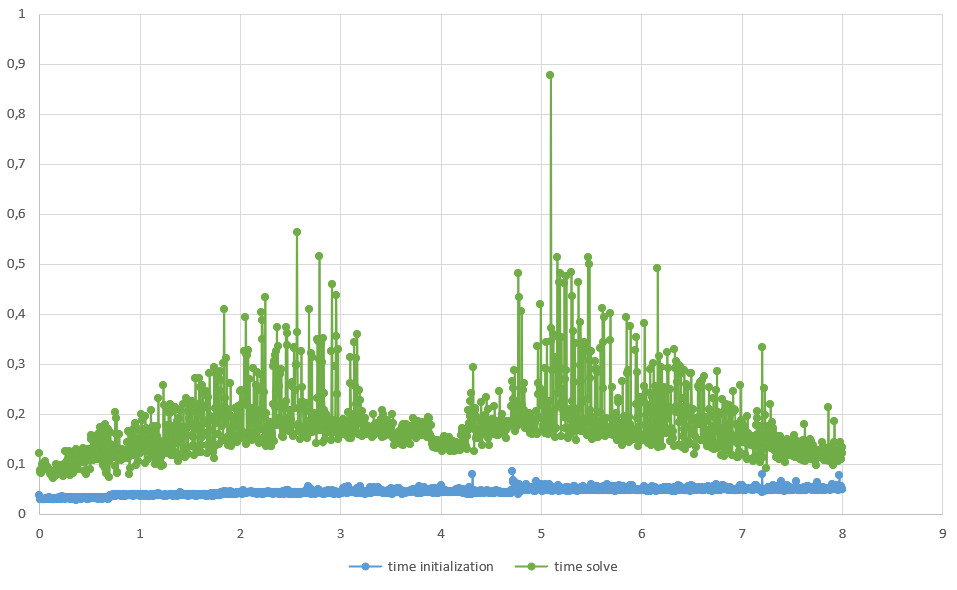
\includegraphics[width=0.6\textwidth]{timings.png}
    \caption{Time taken to initialize the preconditioner and solve the system at each time step.}
\end{figure}

Moving on, the subsequent images illustrate the forces of drag and lift, along with their coefficients, observed over the course of time steps.

\begin{figure}[h]
    \centering
    \begin{minipage}{0.48\textwidth}
        \centering
        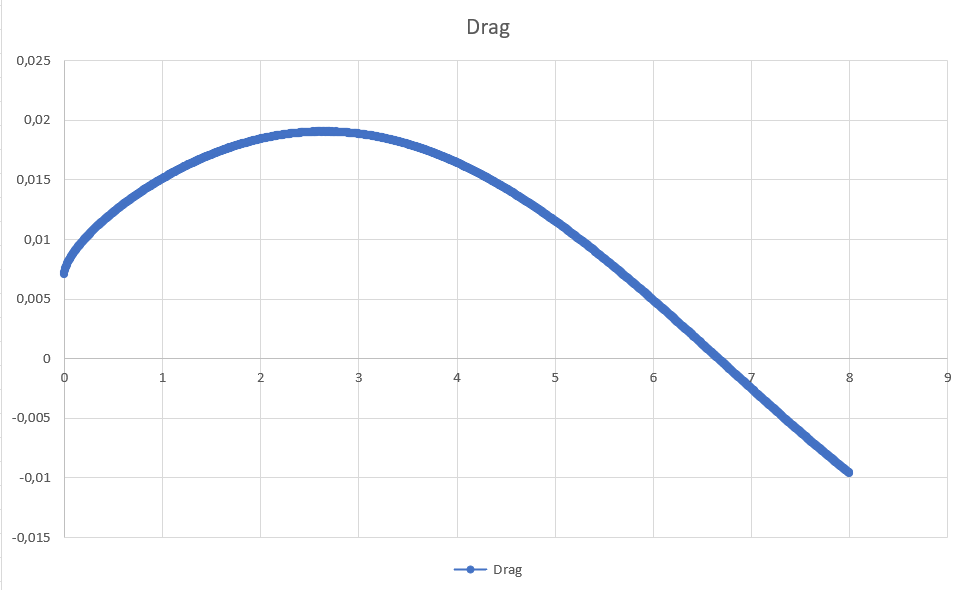
\includegraphics[width=\linewidth]{Drag.png}
        \subcaption{Drag force}
    \end{minipage}\hfill
    \begin{minipage}{0.48\textwidth}
        \centering
        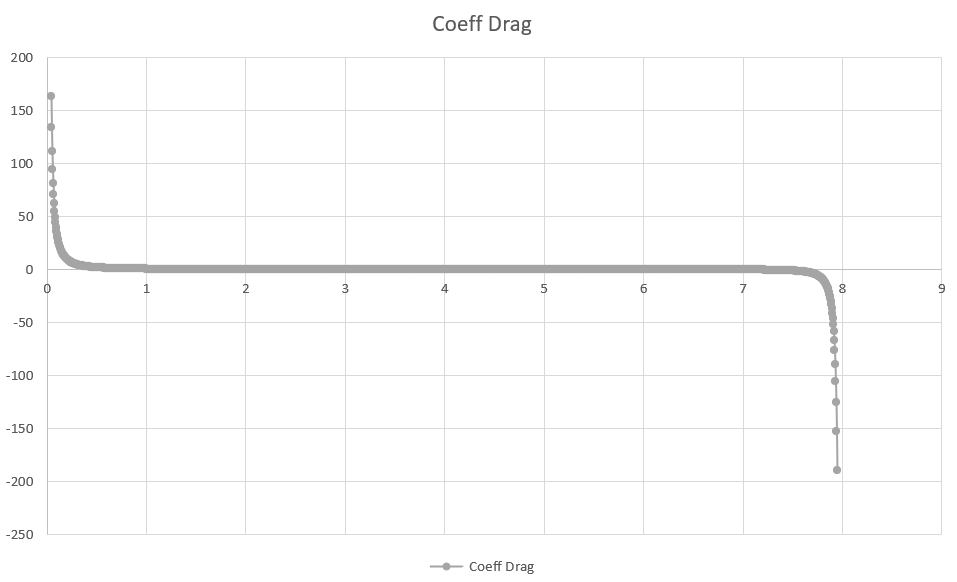
\includegraphics[width=\linewidth]{Coeff_drag.png}
        \subcaption{Drag coefficient}
    \end{minipage}

    \begin{minipage}{0.48\textwidth}
        \centering
        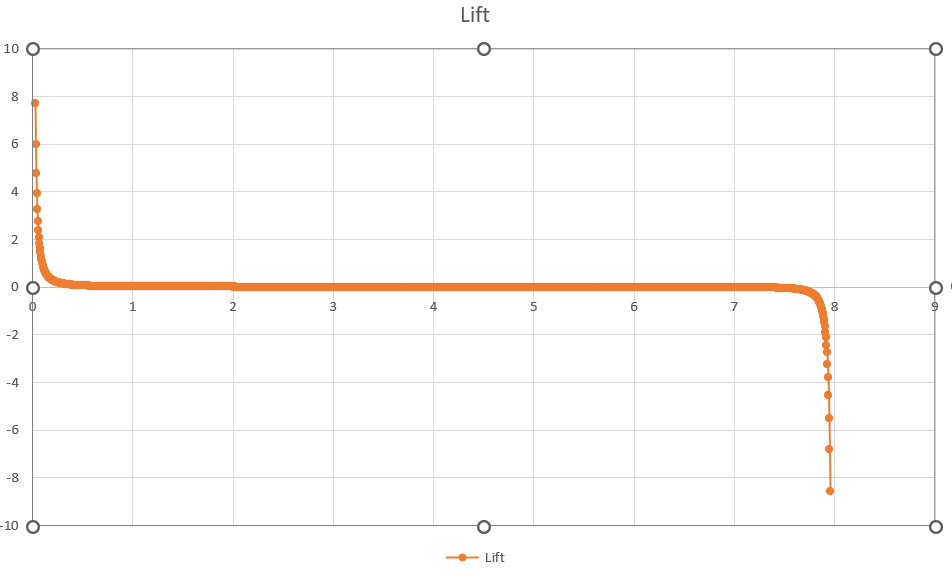
\includegraphics[width=\linewidth]{Lift.png}
        \subcaption{Lift force}
    \end{minipage}\hfill
    \begin{minipage}{0.48\textwidth}
        \centering
        \includegraphics[width=\linewidth]{coeff_lift.png}
        \subcaption{Lift coefficient}
    \end{minipage}

    \caption{Forces of drag and lift over time steps for different cases.}
\end{figure}
Such results, particularly from \(t = 4s\) onward, may be influenced by the fact that the inlet velocity undergoes a gradual decrease, indicating an overall deceleration of the flow throughout the domain. In contrast to the time interval \((0-4]s\), during which the pressure decreases along the x-axis, the pressure exhibits an increasing trend along the x-axis in the later time period. 

Finally, Velocity and pressure transition over time are shown in the groups of figures below:

\begin{figure}
    \centering    
    \subfloat[Velocity at time t=0s]{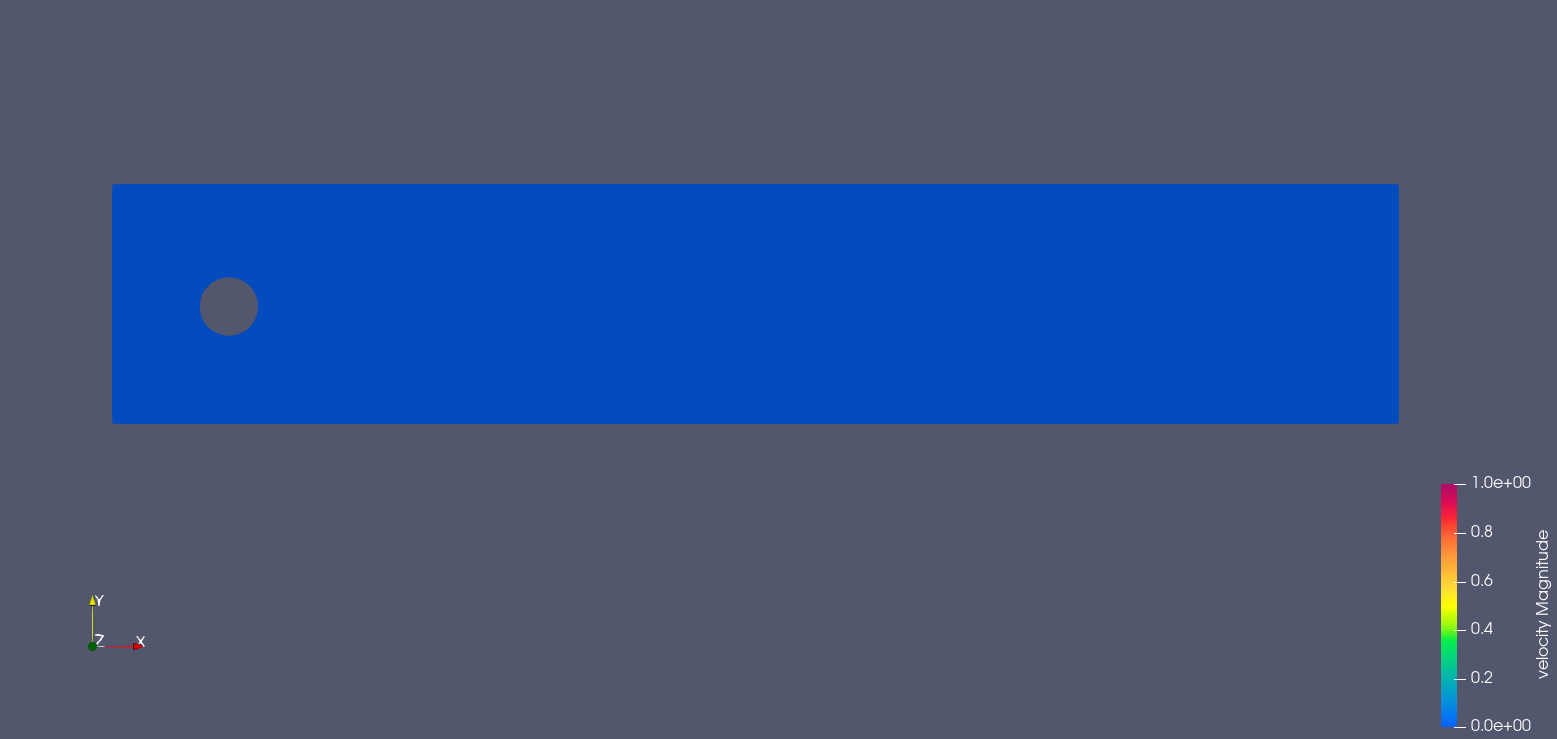
\includegraphics[width=0.5\textwidth]{vtime0.png}\label{fig:sub3}}
    \hfill
    \subfloat[Pressure at time t=0s]{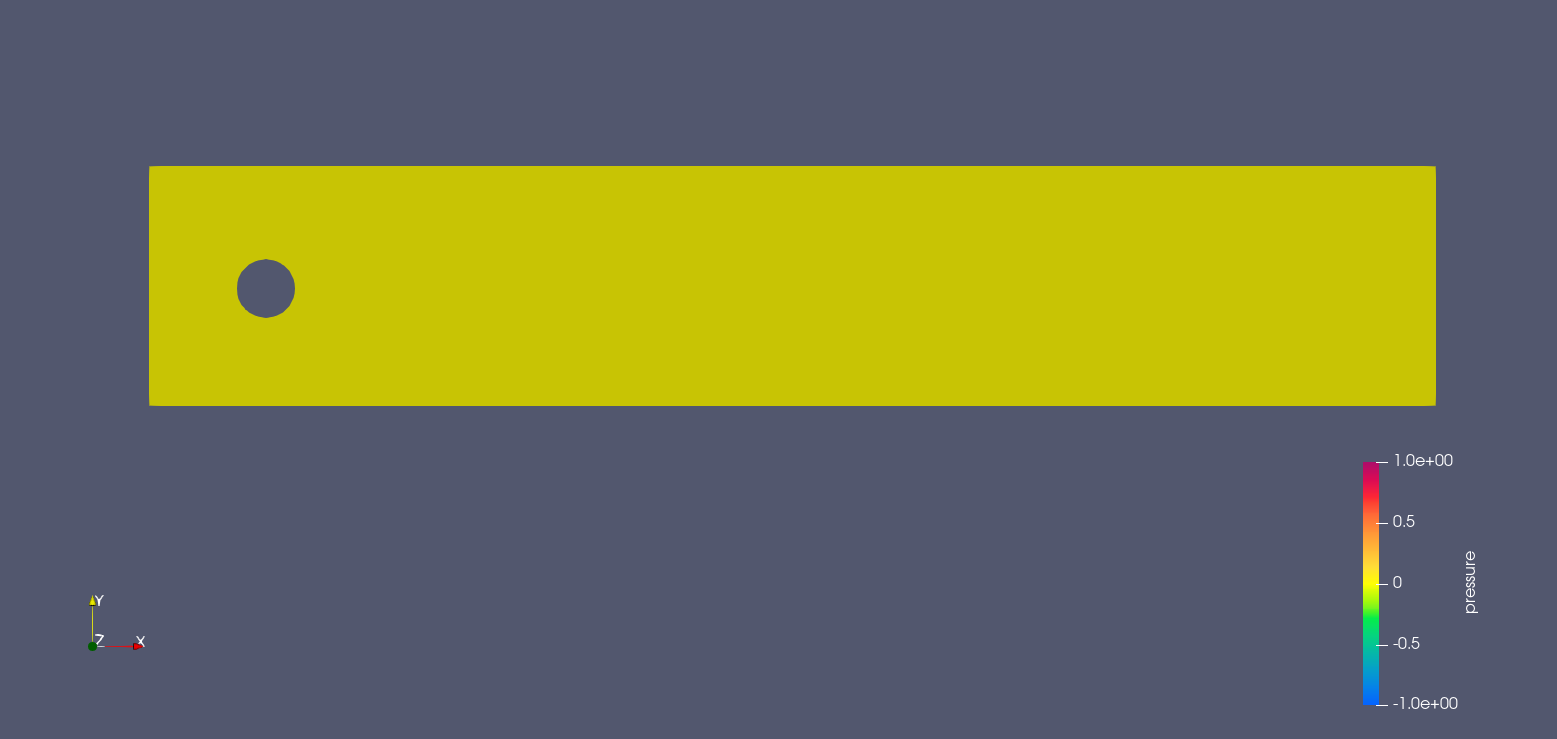
\includegraphics[width=0.5\textwidth]{ptime0.png}\label{fig:sub2}}

    
    \vspace{1em} % Spacing between the rows of images

    \subfloat[Velocity at time t=0.5s]{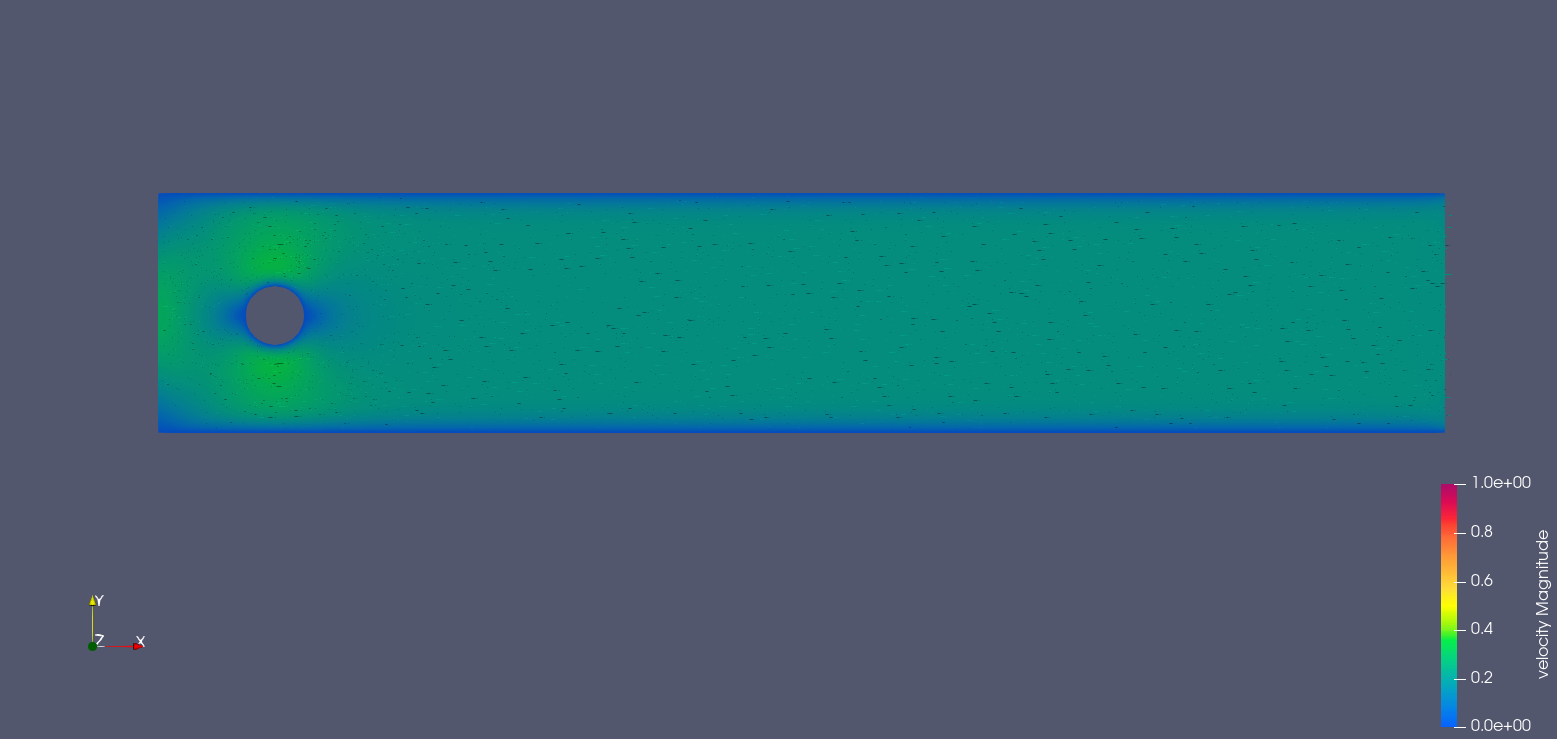
\includegraphics[width=0.5\textwidth]{vtime100.png}\label{fig:sub3}}
    \hfill
    \subfloat[Pressure at time 0.5s]{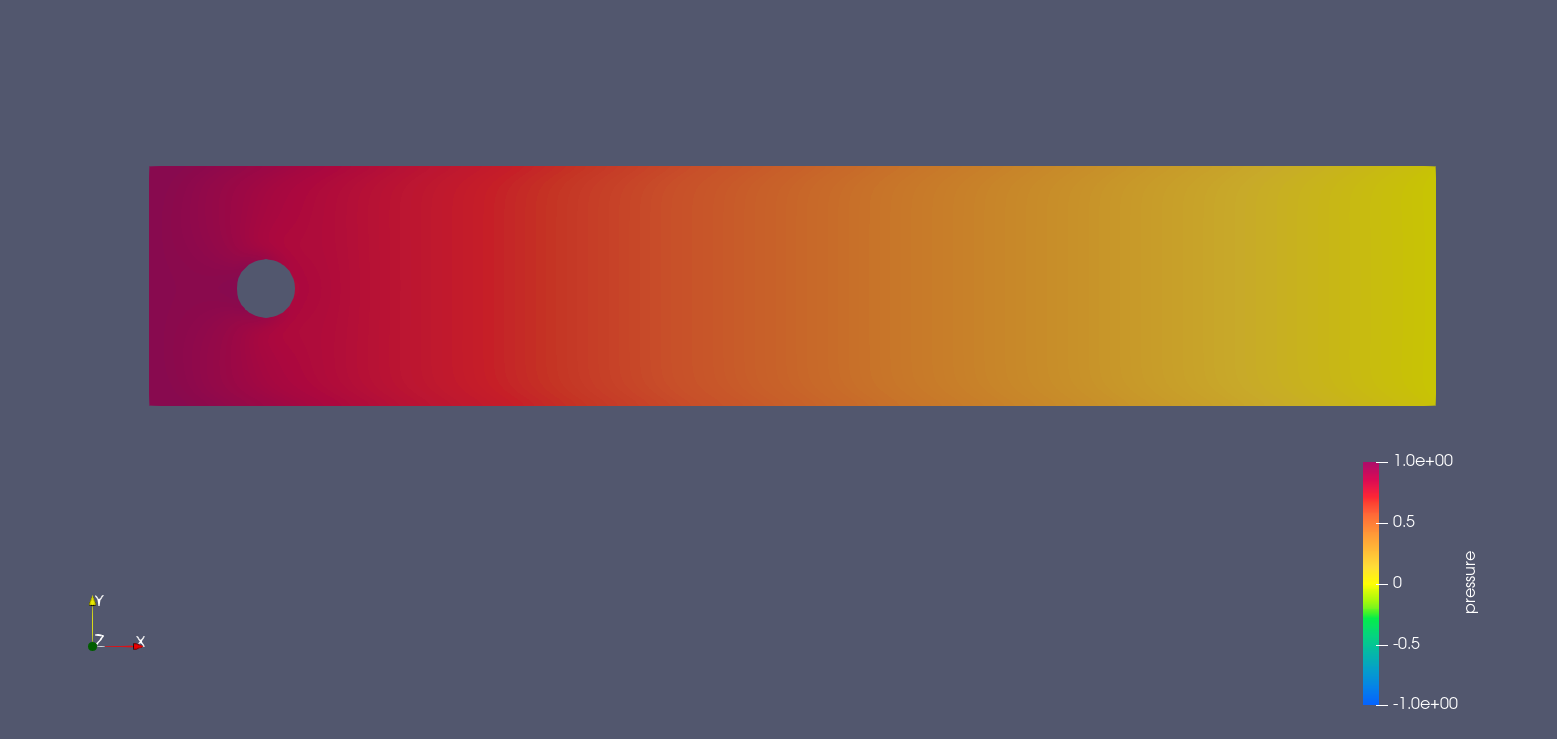
\includegraphics[width=0.5\textwidth]{ptime100.png}\label{fig:sub2}}
    
    \vspace{1em} % Spacing between the rows of images

    \subfloat[Velocity at time t=1.5s]{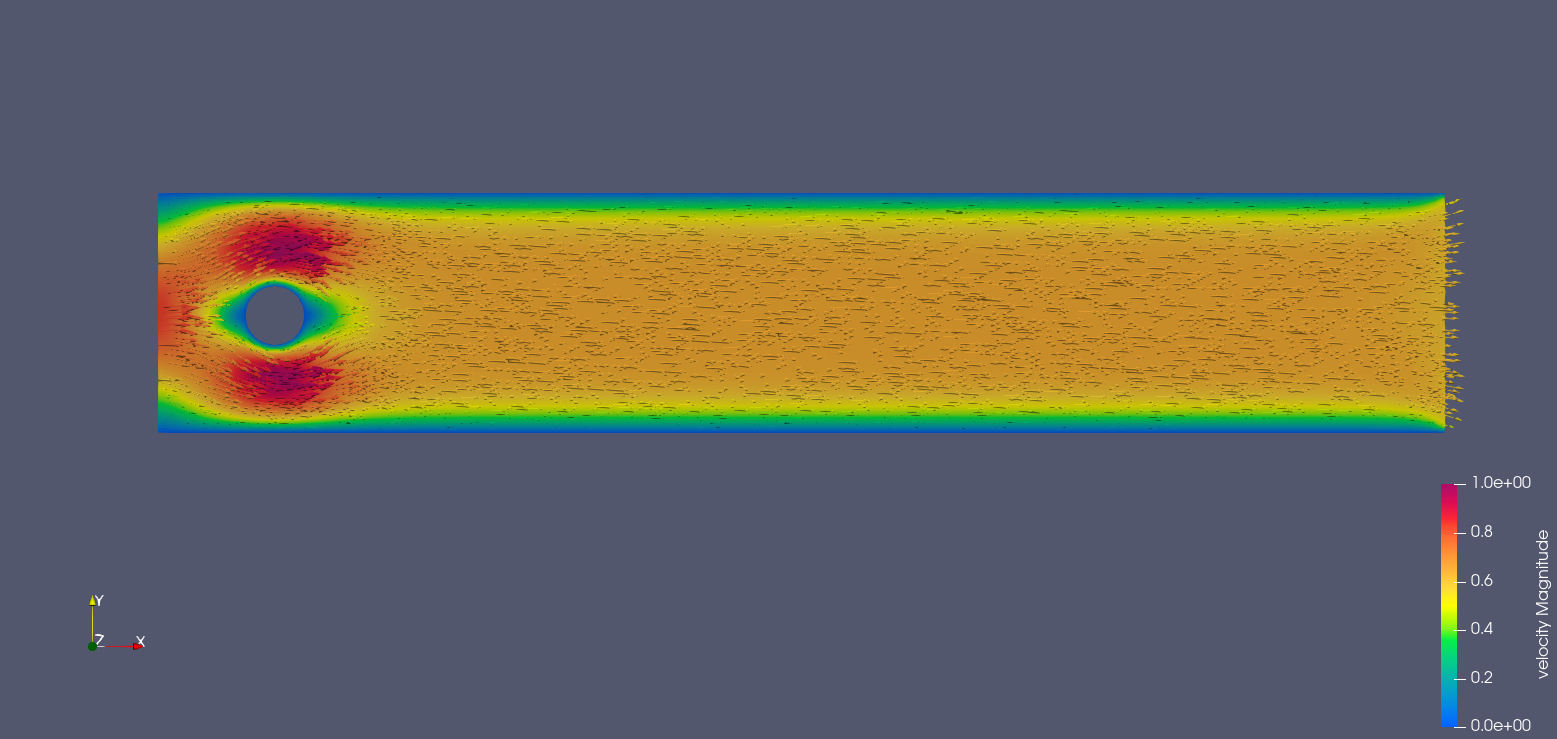
\includegraphics[width=0.5\textwidth]{vtime300.png}\label{fig:sub3}}
    \hfill
    \subfloat[Pressure at time t=1.5s]{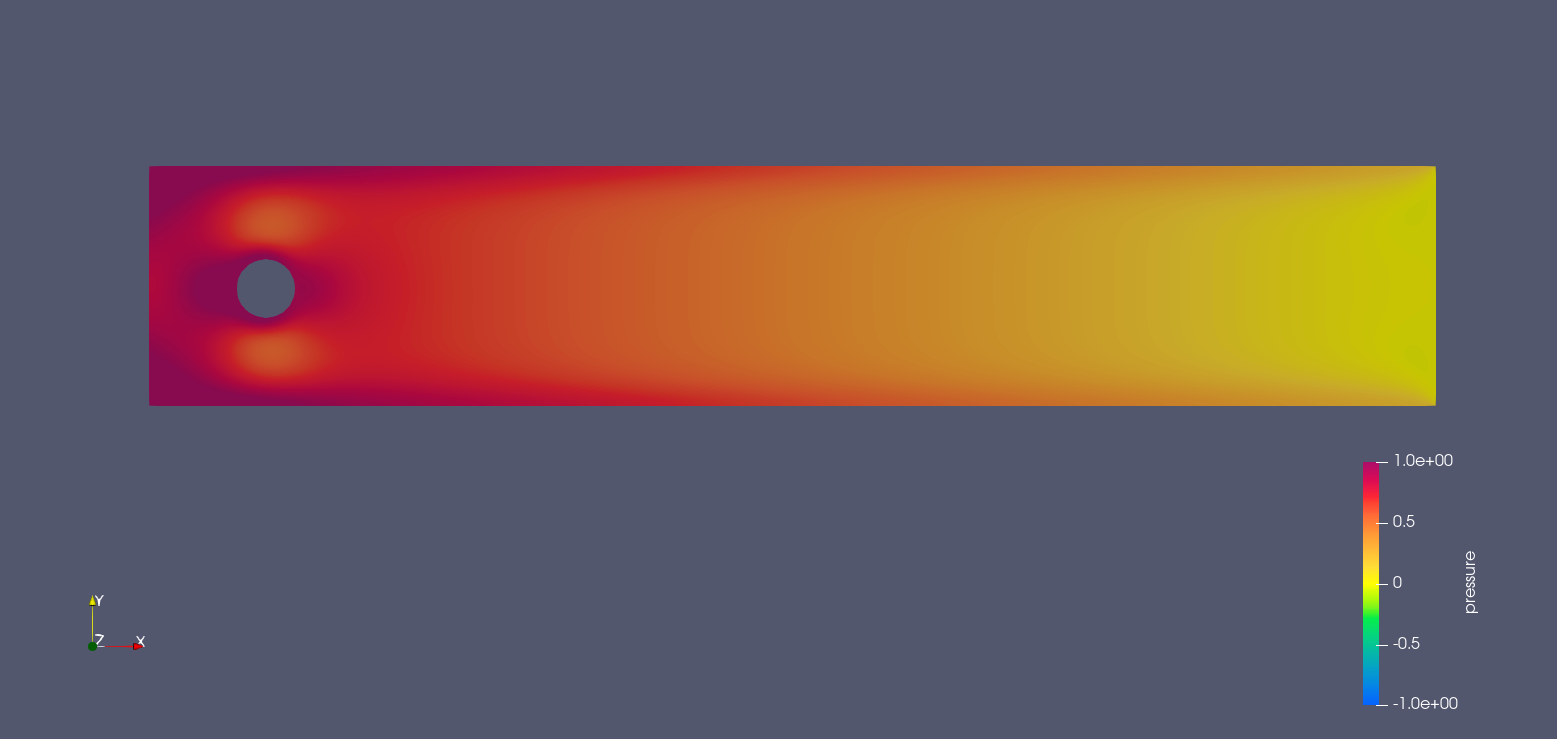
\includegraphics[width=0.5\textwidth]{ptime300.png}\label{fig:sub2}}
    
    \vspace{1em} % Spacing between the rows of images

    \subfloat[Velocity at time \(t=2.0s\)]{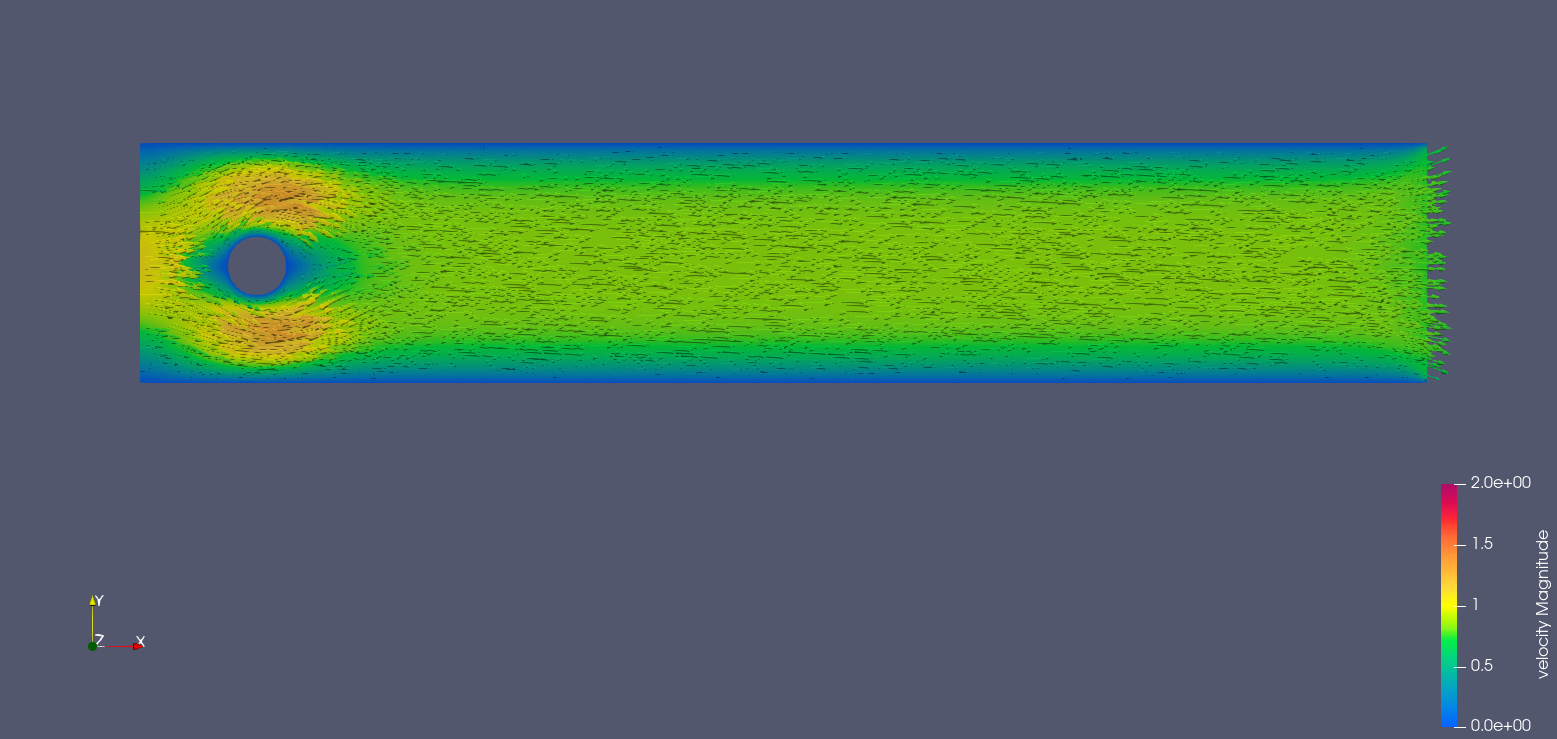
\includegraphics[width=0.5\textwidth]{vtime400.png}\label{fig:sub3}}
    \hfill
    \subfloat[Pressure at time \(t=2.0s\)]{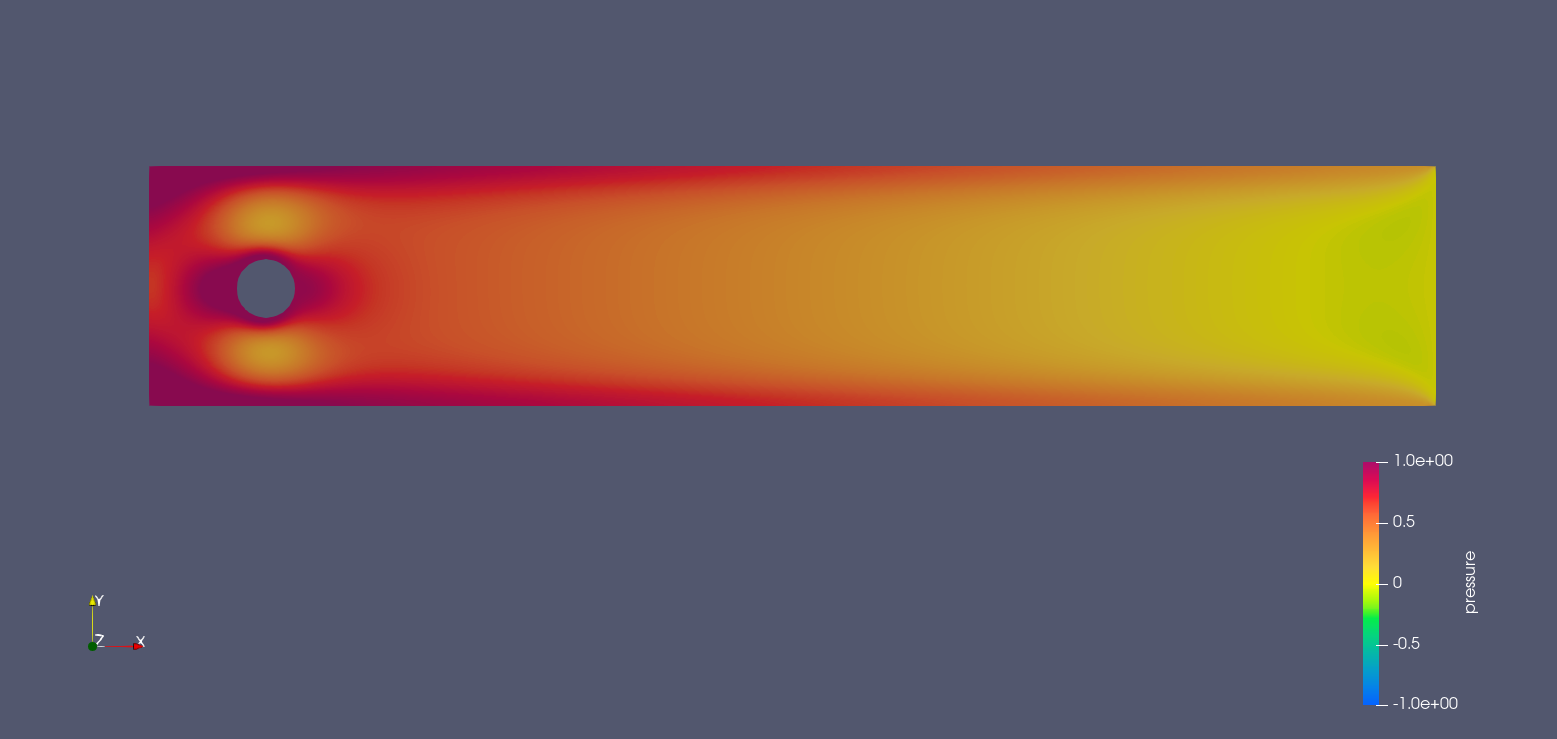
\includegraphics[width=0.5\textwidth]{ptime400.png}\label{fig:sub2}}

    \subfloat[Velocity at time t=2.5s]{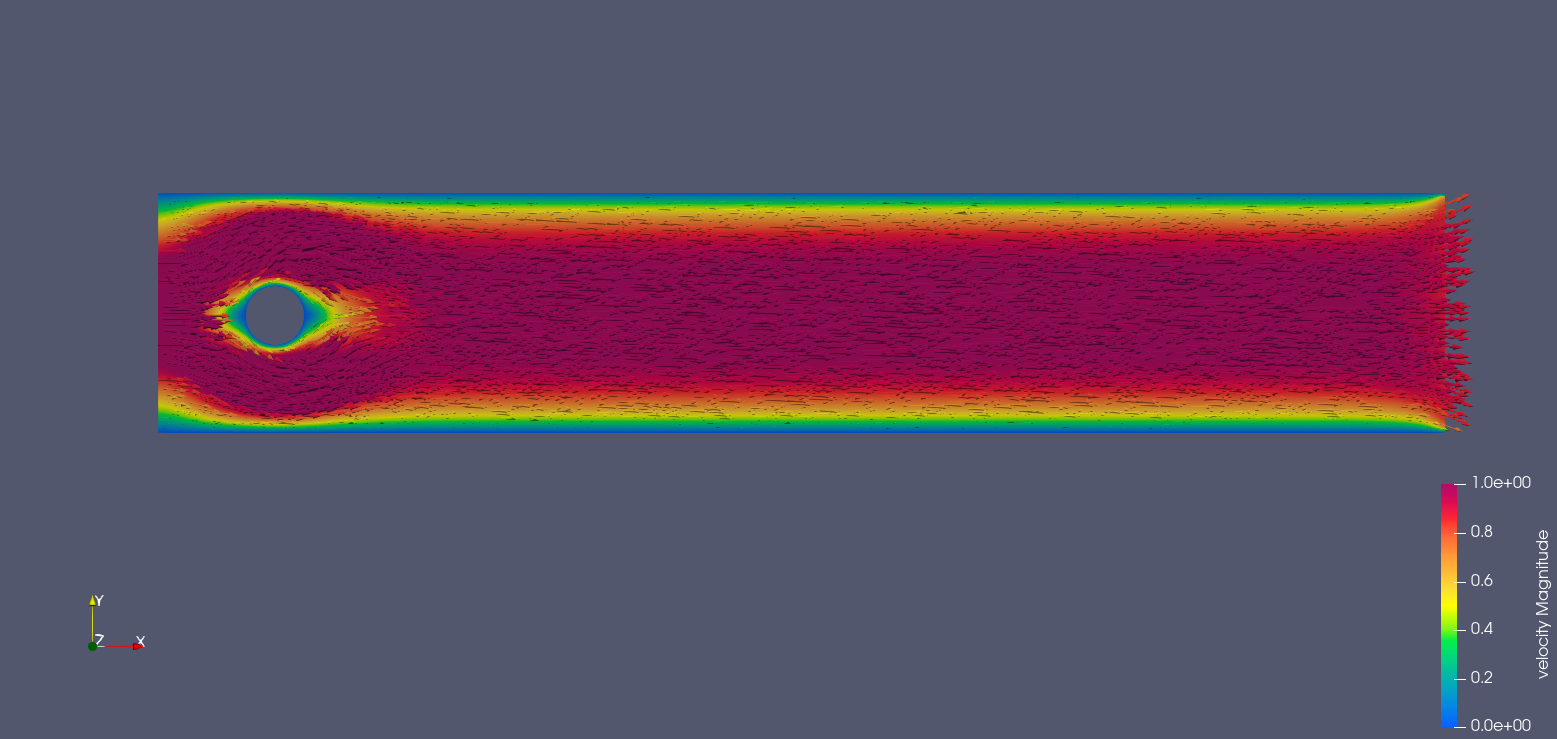
\includegraphics[width=0.5\textwidth]{vtime500.png}\label{fig:sub3}}
    \hfill
    \subfloat[pressure at time t=2.5s]{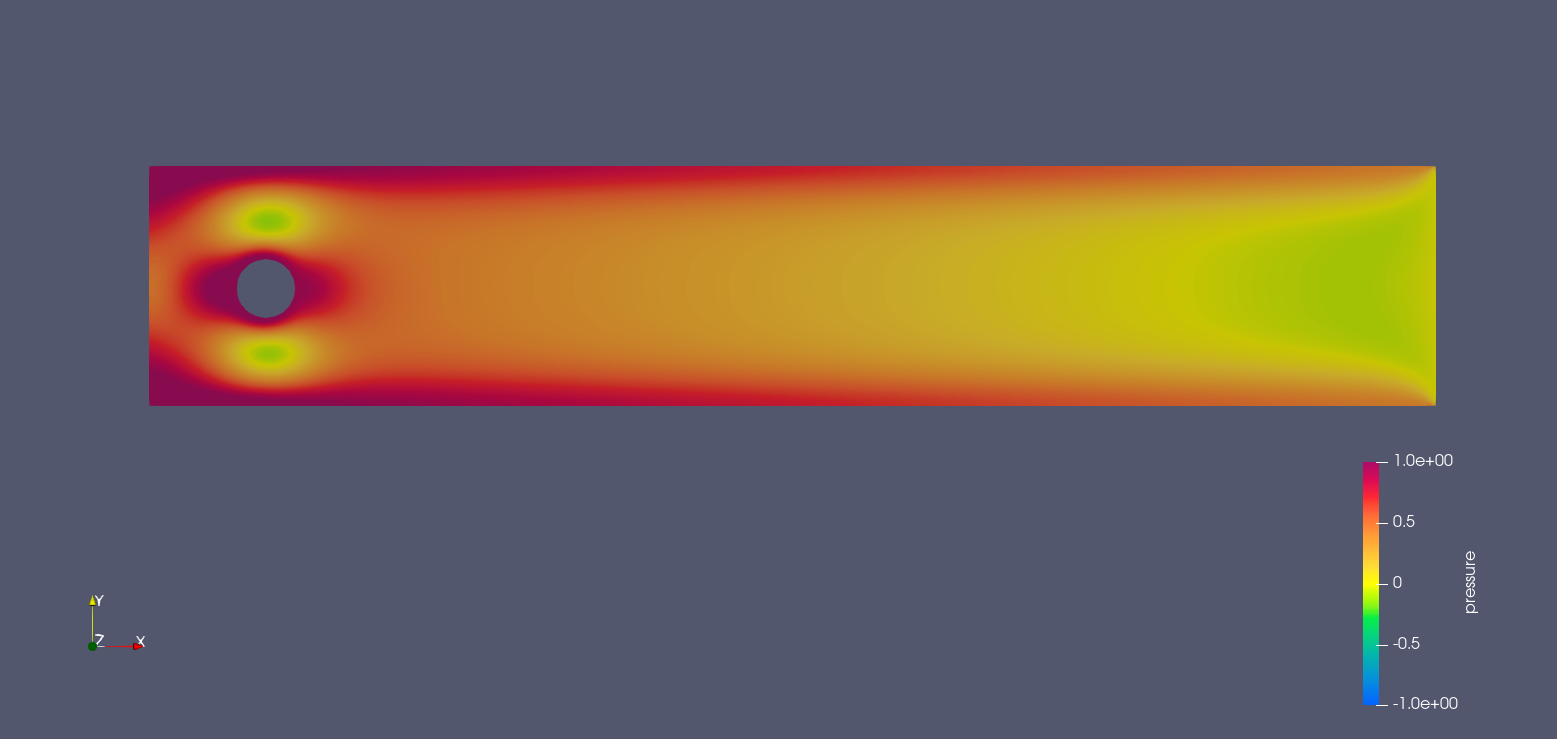
\includegraphics[width=0.5\textwidth]{ptime500.png}\label{fig:sub2}}
    \vspace{1em} % Spacing between the rows of images
    \caption{Velocity and pressure field with accelerating fluid}
    \label{fig:general_label}
\end{figure}

    \vspace{1em} % Spacing between the rows of images
\begin{figure}
\centering
\vspace{1em} % Spacing between the rows of images

    \subfloat[Velocity at time t=3.0s]{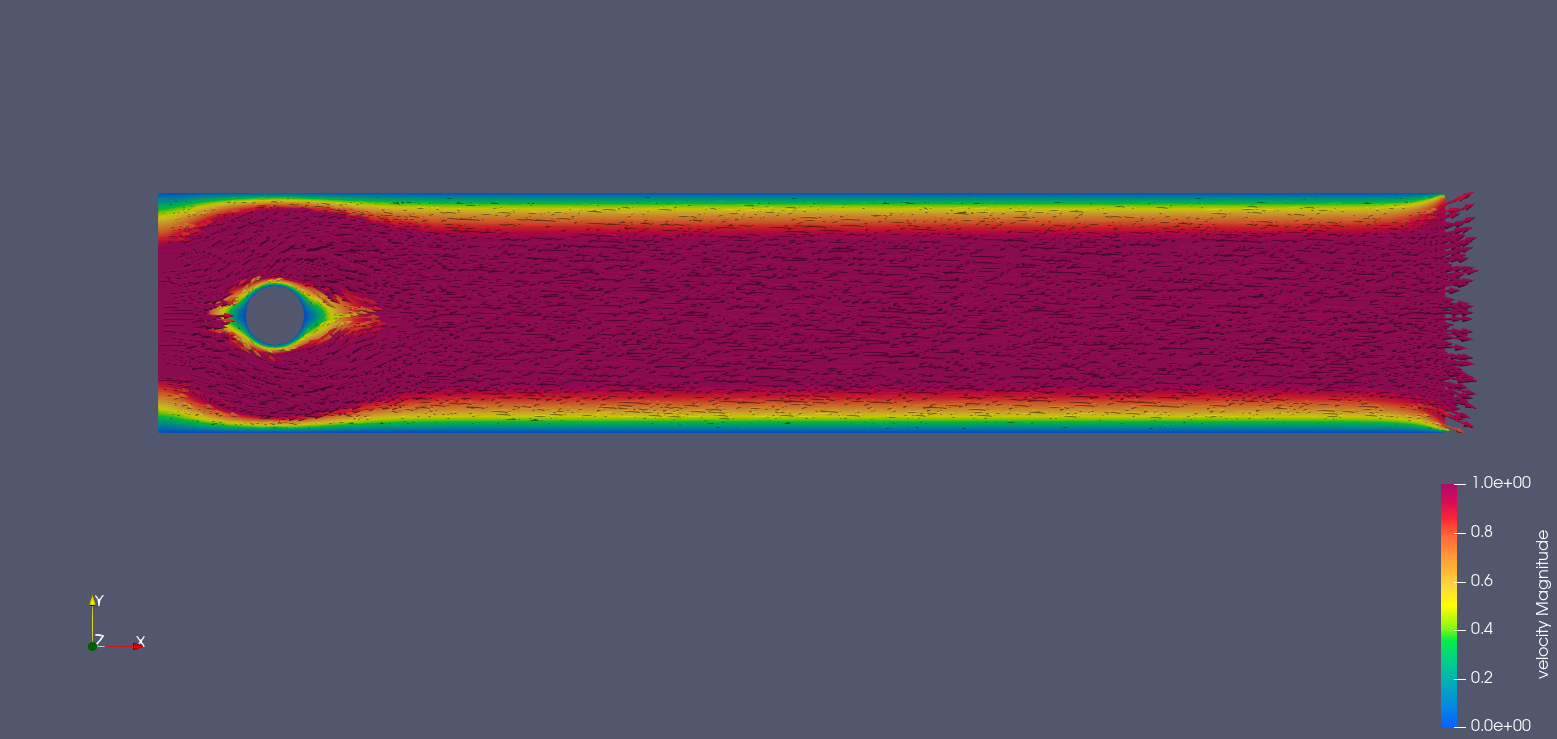
\includegraphics[width=0.5\textwidth]{vtime600.png}\label{fig:sub3}}
    \hfill
    \subfloat[pressure at time t=3.0s]{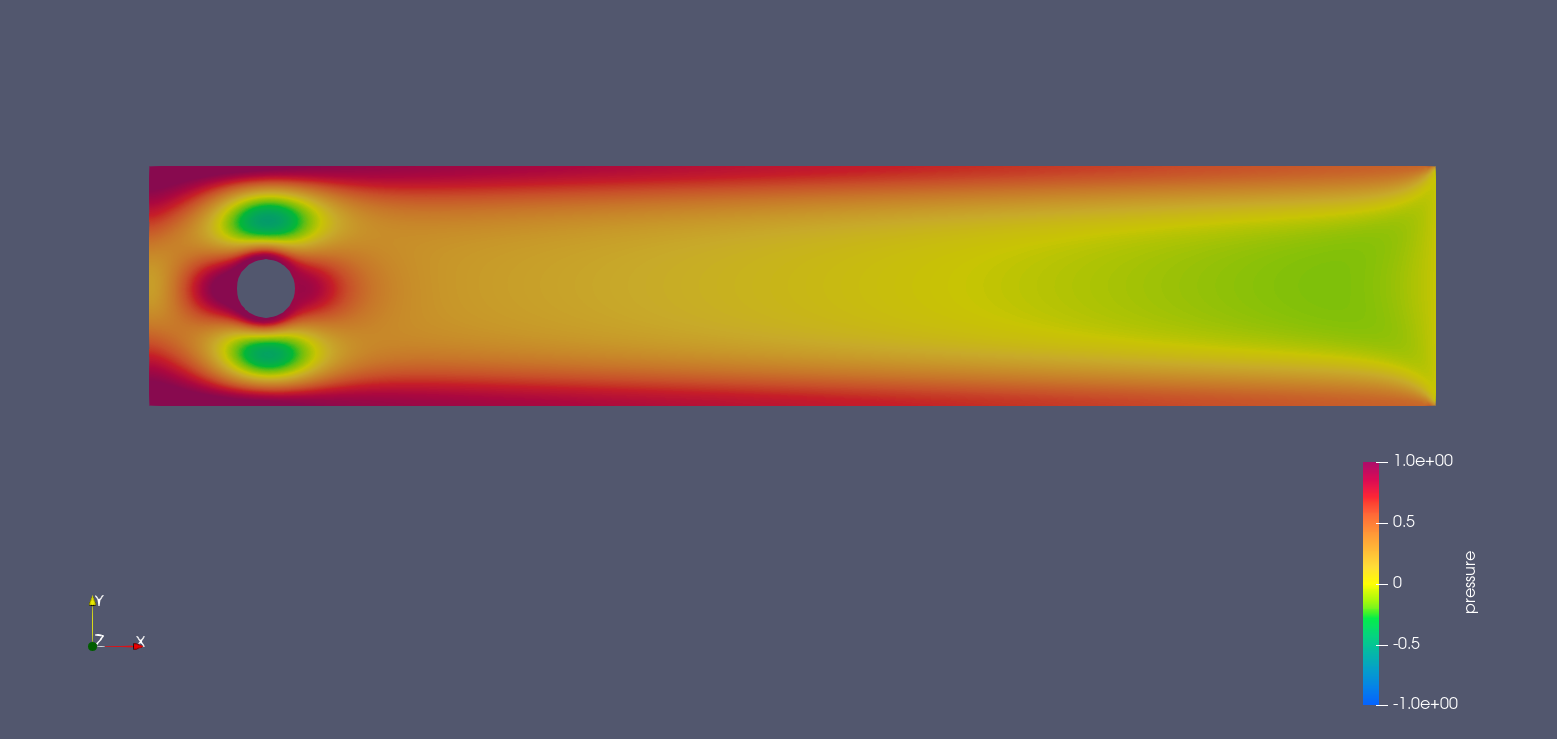
\includegraphics[width=0.5\textwidth]{ptime600.png}\label{fig:sub2}}
    
    \subfloat[Velocity at time t=4.0s]{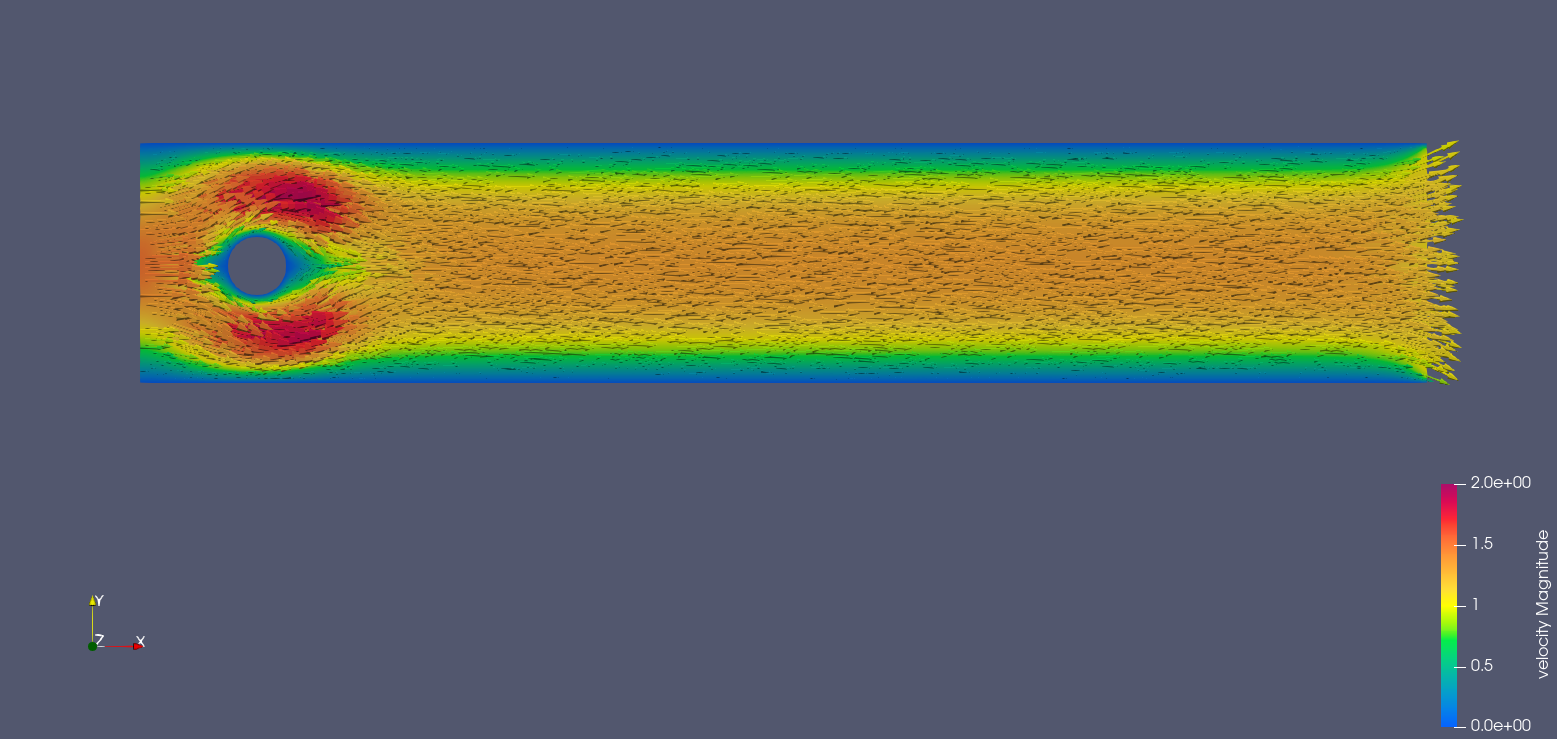
\includegraphics[width=0.5\textwidth]{vtime800.png}\label{fig:sub3}}
    \hfill
    \subfloat[pressure at time t=4.05s]{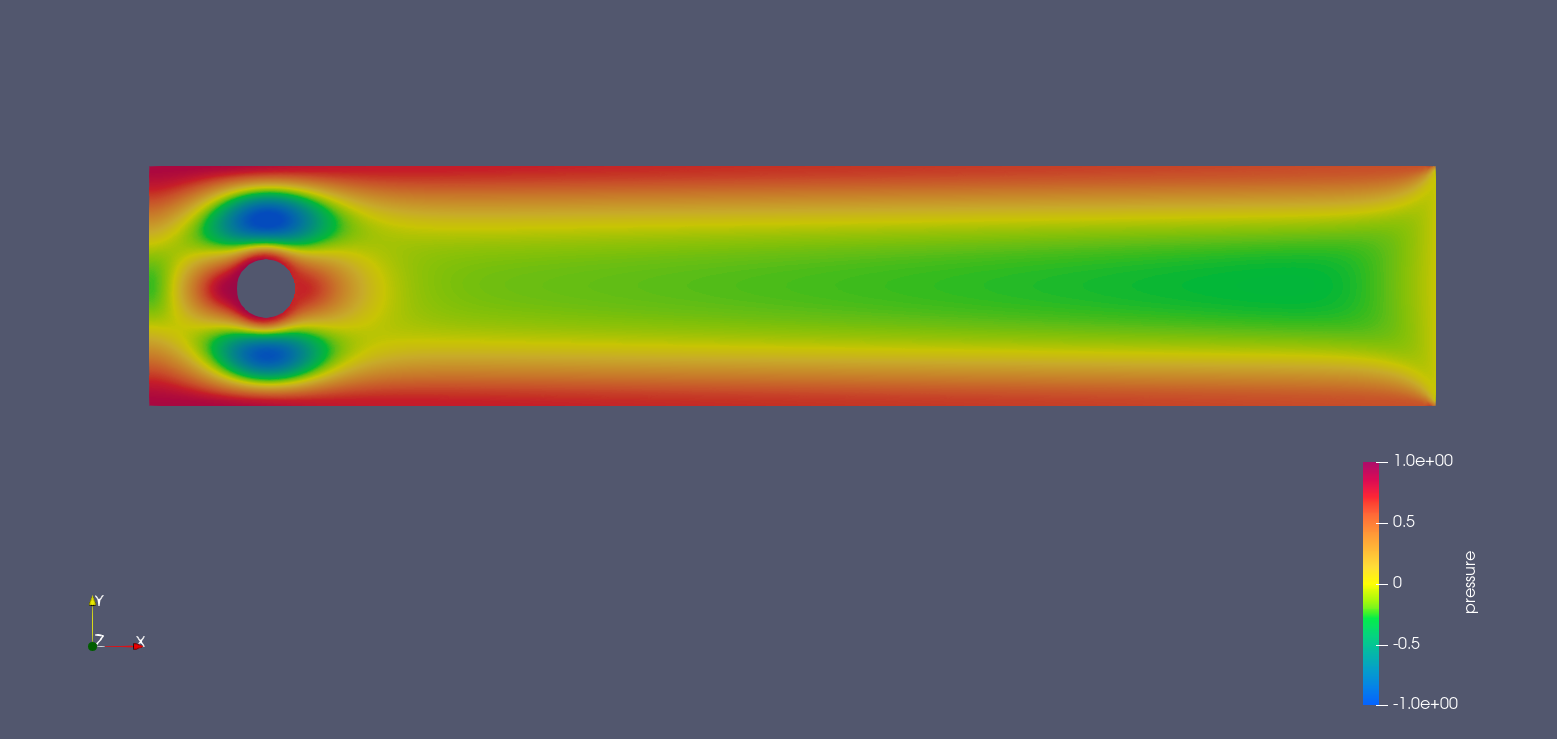
\includegraphics[width=0.5\textwidth]{ptime800.png}\label{fig:sub2}}

    

    \vspace{1em} % Spacing between the rows of images

    \subfloat[velocity at time t=6.0s]{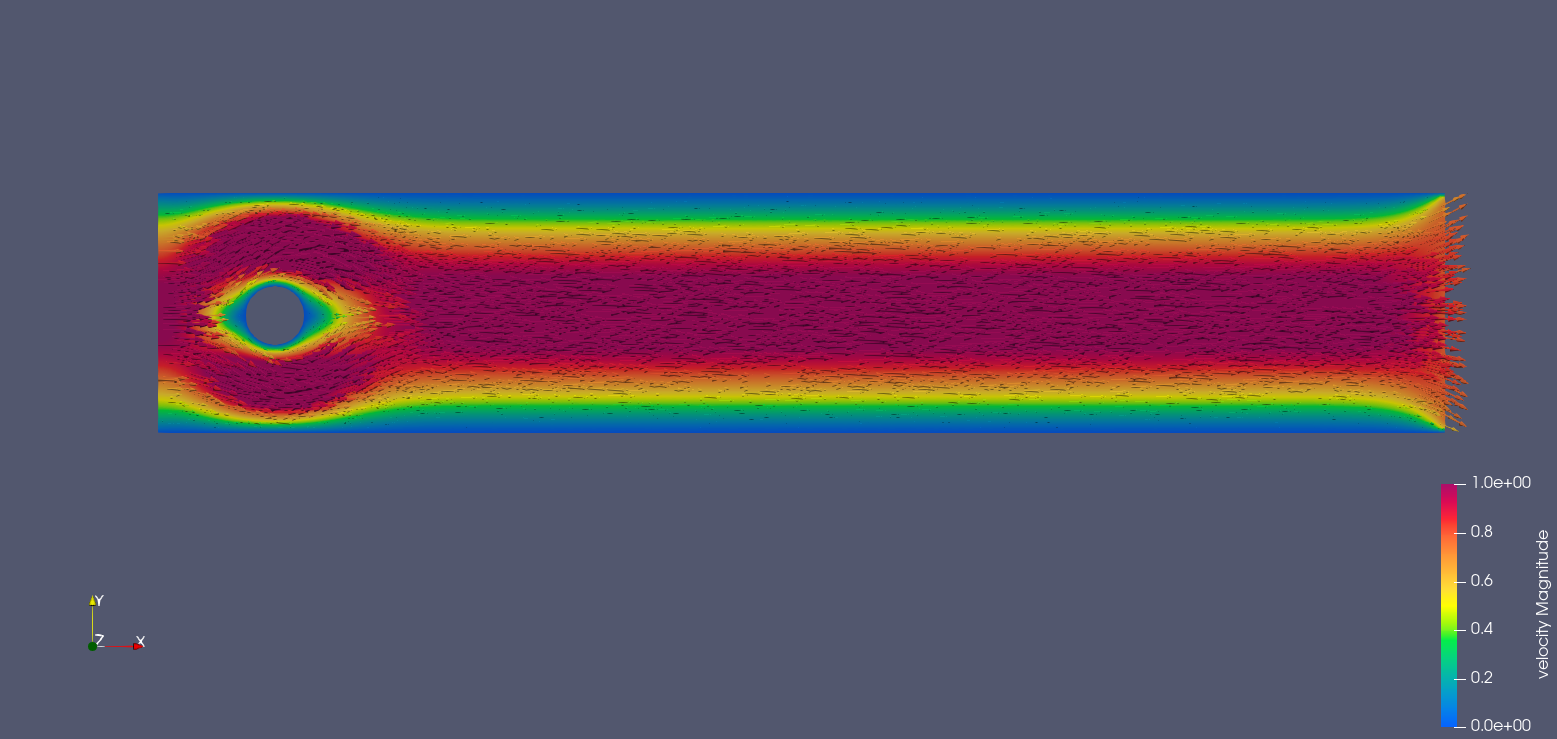
\includegraphics[width=0.5\textwidth]{vtime1200.png}\label{fig:sub3}}
    \hfill
    \subfloat[pressure at time t=6.0s]{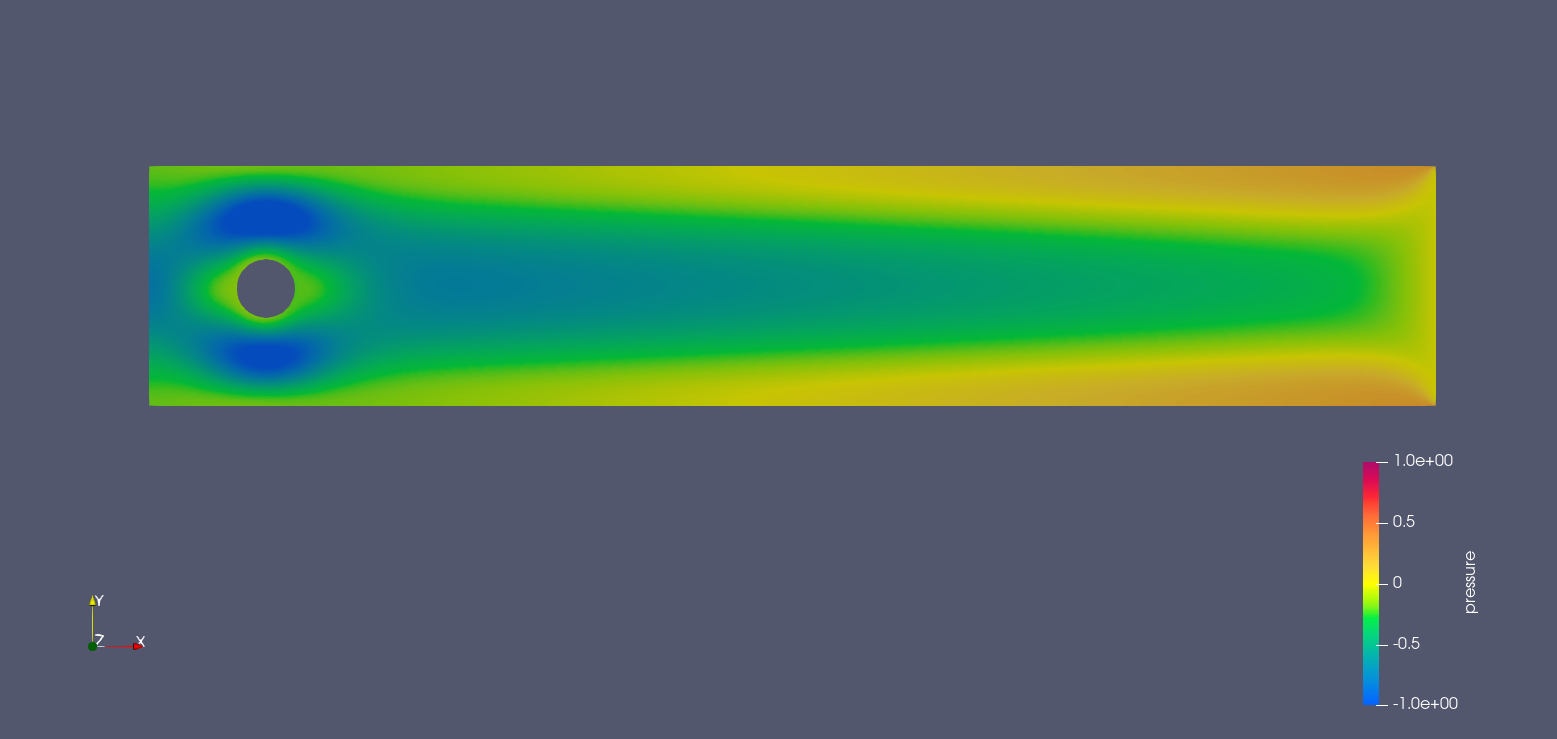
\includegraphics[width=0.5\textwidth]{ptime1200.png}\label{fig:sub2}}
    
    \vspace{1em} % Spacing between the rows of images

    \subfloat[velocity at time t=7.0s]{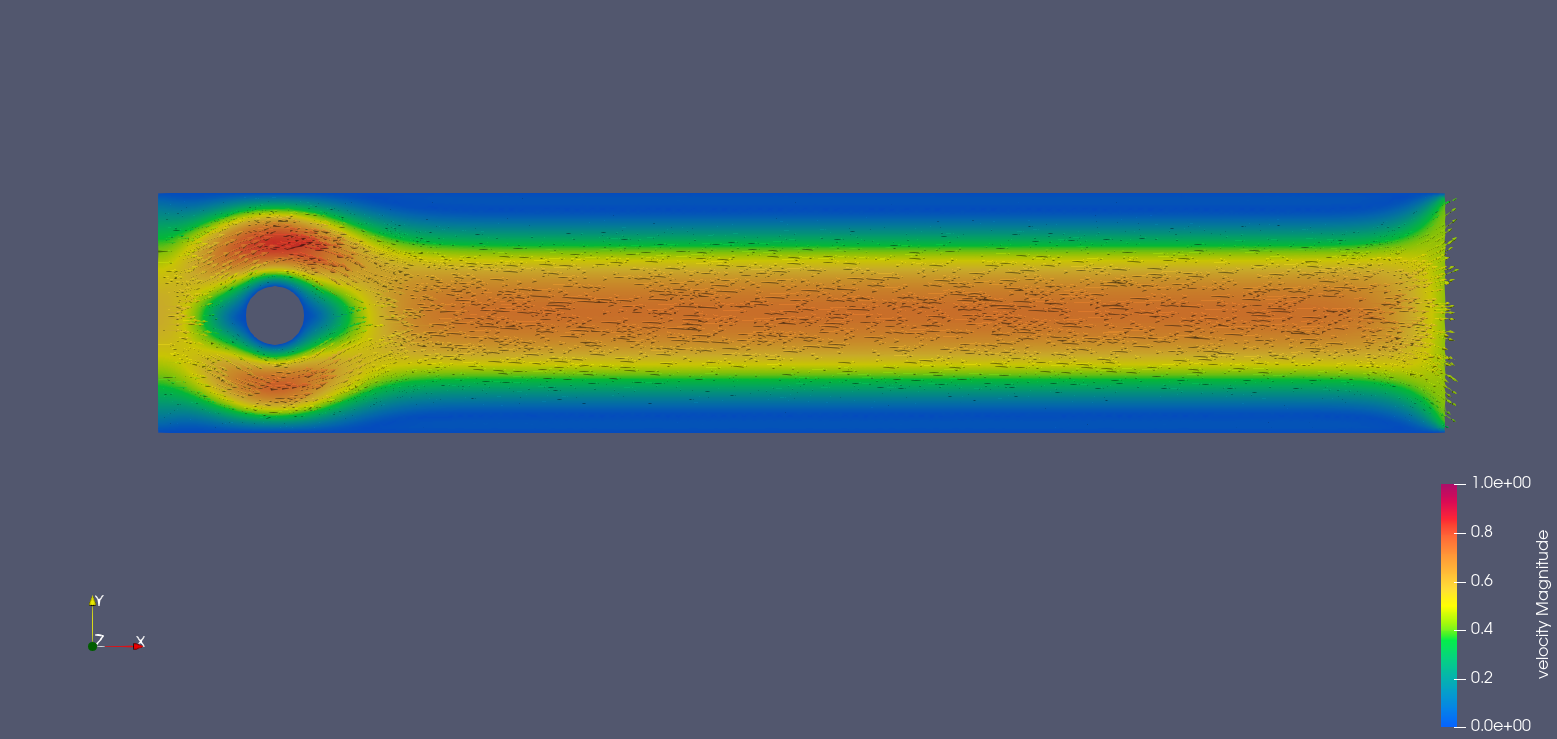
\includegraphics[width=0.5\textwidth]{vtime1400.png}\label{fig:sub3}}
    \hfill
    \subfloat[pressure at time t=7.0s]{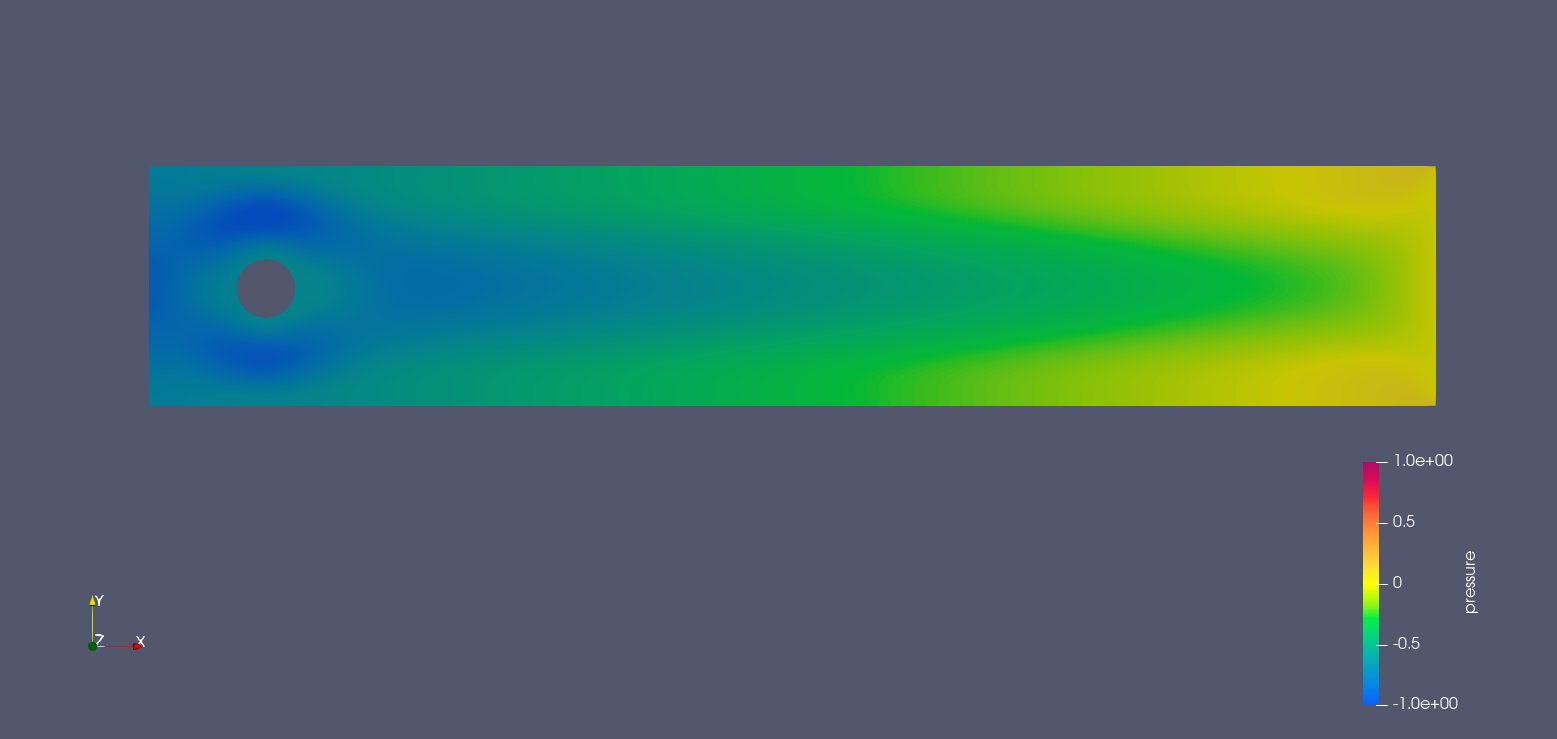
\includegraphics[width=0.5\textwidth]{ptime1400.png}\label{fig:sub2}}

    \subfloat[velocity at time t=8.0s]{\includegraphics[width=0.5\textwidth]{vtime1601.png}\label{fig:sub3}}
    \hfill
    \subfloat[pressure at time t=8.0s]{\includegraphics[width=0.5\textwidth]{ptime1601.png}\label{fig:sub2}}

    \label{fig:P_V_test2}
\end{figure}

\newpage
\subsection{3D Test Cases}
For the 3D test cases, the flows around a cylinder with square and circular cross-sections are considered. The problem configurations and boundary conditions are illustrated in figure \ref{fig:3D}. The outflow condition can be selected by the user. Some definitions are introduced to specify the values that have to be computed. The height and width of the channel are \(H = 0.41 \, \text{m}\), and the side length and diameter of the cylinder are \(D = 0.1 \, \text{m}\). The characteristic velocity is \(U(t) = \frac{4U(0, H/2, H/2, t)}{9}\), and the Reynolds number is defined by \(Re = \frac{UD}{\nu}\). The drag and lift forces are
\begin{align*}
    F_D &= \int_S \left(\rho\nu \frac{\partial v_t}{\partial n}n_y - p n_x\right) \, dS, \\
    F_L &= -\int_S \left(\rho\nu \frac{\partial v_t}{\partial n}n_x + P n_y\right) \, dS,
\end{align*}
with the following notations: surface of the cylinder \(S\), normal vector \(n\) on \(S\) with x-component \(n_x\) and y-component \(n_y\), tangential velocity \(v_t\) on \(S\), and tangent vector \(t = (n_y, -n_x, 0)\). The drag and lift coefficients are
\begin{align*}
    c_D &= \frac{2F_D}{\rho U^2 D H}, \\
    c_L &= \frac{2F_L}{\rho U^2 D H}.
\end{align*}
The Strouhal number is \(St = \frac{Df}{U}\) with the frequency of separation \(f\), and a pressure difference is defined by \(\Delta P = \Delta P(t) = P(x_a, y_a, z_a, t) - P(x_e, y_e, z_e, t)\) with coordinates \((x_a, y_a, z_a) = (0.45, 0.20, 0.205)\) and \((x_e, y_e, z_e) = (0.55, 0.20, 0.205)\).
\subsubsection{Test Cases 3D-1Q and 3D-1Z (Steady)}


The inflow condition is given by:
\[
U(0, y, z) = \frac{16U_m yz (H - y)(H - z)}{H^4}, \quad V = W = 0
\]
with \(U_m = 0.45 \, \text{m/s}\), yielding the Reynolds number \(Re = 20\). 

\subsubsection*{Results}

To solve this problem, we exclusively used the aSIMPLE preconditioner with \(\Delta t = 0.05\) in a time interval \(0 \leq t \leq 8\).

For each time step, we present the time taken to construct the preconditioner, the time taken to solve the problem, and both the drag and lift coefficients. The parallel implementation utilized 5 physical cores, and the tests were conducted on both coarse and fine meshes.

Observations indicate that the time required to build the preconditioner remains consistent, while the time to solve the problem varies significantly, sometimes even becoming smaller then the preconditioner. This variation can be attributed to the steady nature of the problem, where the solution stabilizes over time, necessitating fewer iterations for problem resolution.

No substantial differences were observed elsewhere; the drag and lift coefficients over time remained relatively consistent regardless of the mesh granularity.


\section{Parallelization}

\subsection*{Results}
We conducted multiple runs of Test Case 2D-1 with \(T = 2\), \(\delta t = 0.01\) and the preconditioner aSIMPLE using different processor counts to assess the impact of parallelization on the code's performance. The results are as follows:

\begin{itemize}
    \item [\textbf{6 processors}]: The solution time is 76.4115 seconds, featuring an average preconditioner initialization time of 0.04 seconds and approximately 0.30 seconds for the initial time steps (around 15 GMRES iterations). Notably, the solution time significantly reduces towards the end. Without the preconditioner, the entire system requires about 149.708 seconds to solve. Notably, in the absence of the preconditioner, approximately 28979 iterations are performed in the initial steps, affirming the effectiveness of the preconditioner.

    \item[\textbf{2 processors}]: In this configuration, the solution time is 160.326 seconds. During each time step, approximately 0.1 seconds are spent initializing the preconditioner, and an average of 0.4 seconds is required to solve the problem — still achieved in around 15 iterations.

    \item[\textbf{1 processor}]: Operating the code in serial mode leads to a significant performance decrease, with the total time required to solve the system being 262.893 seconds. The initialization time for the preconditioner increases to around 0.135 seconds at every time step, and an average of 0.6 seconds is needed to solve the system.
\end{itemize}




\begin{thebibliography}{99}
\bibitem{schafer1996}
  Schäfer, S., Turek, F., Durst, F., Krause, E., and Rannacher, R.,
  \emph{Benchmark Computations of Laminar Flow Around a Cylinder},
  Vieweg+Teubner Verlag,
  Wiesbaden,
  1996.

\bibitem{deparis2014}
  Deparis, S., Grandperrin, G., and Quarteroni, A.,
  \emph{Parallel Preconditioners for the Unsteady Navier–Stokes Equations and Applications to Hemodynamics Simulations},
  Computers \& Fluids,
  92:253–273,
  2014.
\end{thebibliography}



\end{document}
